\section{Introduction}
In this chapter, we extend our constraint-based framework to support priority in Reo. 
According to Reo semantics, when several transitions are possible, the network chooses one of them in a non-deterministic fashion. However, in some cases for instance when this non-deterministic choice is between a critical flow and a normal flow, we would like to impose our preference on the non-deterministic choice.  

% Figure \ref{fig:prioritymerger} depicts. The behavior of \emph{priority merger} is defined in terms of coloring semantics.
%
%\begin{figure}[!h]
%\centering
%    \scriptsize
%        \tikz{
%          \node[state] (q) {};
%          \node[state, right of=q, node distance=5cm] (p) {m};
%          \path[transition] (q) edge [loop above] node {$\{\},\textit{true}$} (q); 
%          \path[transition] (q) edge [bend left] node {$\{a, b, e\},\hat{a}=\hat{b} \wedge \hat{b}=\hat{e} \wedge \hat{m}'=\hat{e}$}  (p);     
%          \path[transition] (q) edge [bend right] node {$\{c,d,e\},\hat{d}=\hat{e} \wedge \hat{m}'=\hat{e}$}  (p);
%          \path[transition] (p) edge [loop above] node {$\{\},\textit{true}$} (p); 
%          \path[transition] (p) edge  node {$\{f\}, \hat{m}=\hat{f}$}  (q);                            
%        }
%   \label{fig:prioritymerger}
%   \caption{Priority Merger}
%\end{figure}
%
%Addressing priority as a distinct concept from context-sensitivity in Reo networks requires explicit notion. 
%Arbab et al. ~\cite{priority} introduce several channels to incorporate in the open-ended set or Reo channels that provide an expressive framework to allow imposing, propagating and blocking the priority and its propagation. 

Arbab et al. in ~\cite{priority} introduce a compositional approach to model priority and a priority-aware formal semantics for Reo, named Constraint Automata with Priority (CAP), which is an extension of constraint automata.

Their approach, which distinguishes between where priority is originated from and where it must be applied i.e. non-deterministic choices, consists of the following elements:

\begin{itemize}
 \item A primitive to impose priority that is \emph{PrioritySync},
 \item A mechanism to propagate priority from the location it is imposed through the network,
 \item A mechanism to block the propagation of priority in desired places using one of the following primitives:  
 \begin{itemize}
 \item \emph{BlockSourceSync}, which stops propagation of priority coming from its source end toward its sink;
 \item \emph{BlockSinkSync}, which blocks propagation of priority from its sink end toward its source; 
 \item \emph{BlockSync} that stops propagation of priority on both ends.
 \end{itemize}
\item Means to affect the otherwise non-deterministic choices by priority.
\label{item:prioreq}
\end{itemize}

CAP is an expressive formalism for supporting priority in Reo. However, its operations to manipulate CAPs are computationally expensive, if they are implemented in a straight-forward fashion. Moreover, similar to CA, CAP does not formalize existence of I/O requests on nodes, which is referred to as context. Context is needed to explicitly express conditions in which a transition of higher priority is not feasible due to lack of request; and therefore, a lower priority transition occurs.   

We overcome these shortcomings by extending our constraint-based framework with priority encoding constraints. Our approach %constraint framework to obtain priority-aware semantics of Reo connectors
 benefits from efficient optimized off-the-shelf constraint solvers. Since the framework already includes connector coloring semantics, by reflecting context information in constraints that describe behavior of a Reo connector, we can explicitly express aforementioned conditions. %This explicit information is useful for instance in analyzing and  executing Reo connectors. 
 
Our approach consists of the following elements:
 
 \begin{itemize}
 	\item We use the \emph{PrioritySync} primitive to impose priority, 
 	\item We present a model to propagate the priority through the network that is similar to connector coloring semantics,
 	\item We use \emph{BlockSourceSync}, \emph{BlockSinkSync}, and \emph{BlockSync} to block the propagation of priority in desired places,
	\item We extend our constraint-based framework to incorporate the propagated priority information.
 \end{itemize}
 
%The rest of this chapter presents our approach in providing a priority-aware formal semantics for Reo. 

\section{Priority as Constraint}
In this section, we introduce a model inspired by the coloring semantics \cite{coloring} for presenting propagation of priority within a Reo network. Similar to CAP, we distinguish between two types of priority on a node:

\begin{itemize}
\item
 when the node is imposing the priority to be propagated, which we call it \emph{innate} priority, 
\item when the node has obtained the priority through propagation, we refer to it as $acquired$. 
\end{itemize}

We utilize three colors $\bullet$, $\circ$, and $\times$ to denote \emph{innate} priority, \emph{acquired} priority, and lack of priority, respectively.

Let $\mathcal{N}$ be a set of Reo nodes and $\mathcal{C}$ be the set of colors $\bullet$, $\circ$, and $\times$.

\begin{definition}[Priority Coloring Function]
A priority coloring function $p : N \rightarrow \mathcal{C}$ for $N \subseteq \mathcal{N}$ maps
a node to a color, which expresses the priority status of that node.%Rephrase
\end{definition}

\begin{definition}[Priority Coloring Table]
 A priority coloring table, $P$, over nodes $N \subseteq \mathcal{N}$ is a set of priority colorings on $N$, which we refer to it the domain of $P$.
%rephrase ghablesho
\end{definition}%rephrase

To compute the priority coloring of a connector, we need to compose the priority colorings of its elements using  the join operator, denoted by $\infty$. %, whose definition follows.

\begin{definition}[Priority Join]
We define the join of two coloring tables $P_1$ and $P_2$ with distinct domains $N_1$ and $N_2$ on the connecting nodes $n_1 \in N_1$ and $n_2 \in N_2$ as:

$$P_1 \infty_{n_1, n_2} P_2 = \cup_{(p_1, p_2) \in P_1 \times P_2, n \in N_1 \cup N_2} p_1 \infty_{n_1, n_2} p_2(n)$$
where,
$$p_1 \infty_{n_1, n_2} p_2(n) = \longtwopartdef{n \in N_1}{p_1(n)}{n \in N_2}{p_2(n)}$$

%For all coloring tables $p_1 \in P_1, p_2 \in P_2: p_1 \cup p_2  \in P_1 \infty_{n_1, n_2} P_2 $ 

iff one of the following conditions holds:

\begin{enumerate}
\item $p_1(n_1)=\times \wedge \ p_2(n_2)=\times$
\item $p_1(n_1)=\circ \wedge \ p_2(n_2)=\bullet$
\item $p_1(n_1)=\bullet \wedge \ p_2(n_2)=\circ$
\item $p_1(n_1)=\bullet \wedge \ p_2(n_2)=\bullet$
\end{enumerate}
\label{def:priojoinoperator}
\end{definition}

Table \ref{tab:firstpriocol} shows  the priority coloring of some commonly used Reo channels.

\begin{longtable}{|c|c|c|}
\caption{Priority Coloring of commonly used Reo Primitives} \label{tab:firstpriocol}
  \\ \hline
%r1c1
	\begin{minipage}[t]{.3\linewidth}
         \centering
         \begin{tabular}{c}
               \tikz{
          	   \node[point,label=left:$a$] (A) {};
           	   \node[point,right of=A,label=right:$b$, node distance=8mm] (B) {};
           	   \draw[sync] (A) -- (B);
           	   \node[] at (.4,0) {$!$};}
	    \vspace{0cm}
            \end{tabular}\hfill \newline
            \centering
         \begin{tabular}{|c|c|}
             \hline
               a & b \\
            \hline
              $\bullet$ & $\bullet$ \\ 
            \hline
         \end{tabular}
         \vspace{.3cm}
   \end{minipage}
		&
               % row 1 cell 2
           \begin{minipage}[t]{.3\linewidth}
         \centering
             \tikz{
          	   \node[point,label=left:$a$] (A) {};
           	   \node[point,right of=A,label=right:$b$, node distance=8mm] (B) {};
           	   \draw[sync] (A) -- (B);
           	   \node[] at (.4,0) {$)$};}
	    \vspace{.3cm}
   \\
         \centering
         \begin{tabular}{|c|c|}
             \hline
               a & b \\
            \hline
              $\times$ & $\times$ \\ 
            \hline
              $\circ$ & $\times$ \\
            \hline
              $\circ$ & $\circ$ \\ 
            \hline
         \end{tabular}
          \vspace{0cm}
    \end{minipage}  &
          %row 1 cel 3
             \begin{minipage}[t]{.3\linewidth}
         \centering
             \tikz{
          	   \node[point,label=left:$a$] (A) {};
           	   \node[point,right of=A,label=right:$b$, node distance=8mm] (B) {};
           	   \draw[sync] (A) -- (B);
           	   \node[] at (.4,0) {$($};}
	    \vspace{0cm}
         \\
         \vspace{0cm}
         \centering
            \begin{tabular}{|c|c|}
		\hline
			a & b \\
		\hline
			$\times$ & $\times$ \\ 
		\hline
			$\times$ & $\circ$ \\
		\hline
			$\circ$ & $\circ$ \\ 
		\hline
	\end{tabular}
    \end{minipage}
 
  \\ \hline

             \begin{minipage}[t]{.3\linewidth}
              \centering
                        \tikz{
          	   \node[point,label=left:$a$] (A) {};
           	   \node[point,right of=A,label=right:$b$, node distance=8mm] (B) {};
           	   \draw[sync] (A) -- (B);
           	   \node[] at (.4,0) {$)($};}
	    \vspace{0cm}
        \centering    \\
        \begin{tabular}{|c|c|}
		\hline
			a&  b\\
		\hline
			$\times$ & $\times$ \\ 
		\hline
			$\times$ & $\circ$  \\ 
		\hline
			$\circ$ & $\times$ \\ 
		\hline
			$\circ$ & $\circ$  \\
		\hline
	\end{tabular}
	         \vspace{.1cm}
    \end{minipage}    	&
    \begin{minipage}[t]{.3\linewidth}
              \centering
         \begin{tabular}{c}
               \tikz{
          	   \node[point,label=left:$a$] (A) {};
           	   \node[point,right of=A,label=right:$b$, node distance=8mm] (B) {};
           	   \draw[sync] (A) -- (B);}
            \end{tabular}
            \vspace{0cm} \newline
         \centering
            \begin{tabular}{|c|c|}
		\hline
			a & b \\
		\hline
			$\times$ & $\times$ \\ 
		\hline
			$\circ$ & $\bullet$ \\ 
		\hline
			$\bullet$ & $\circ$ \\ 
		\hline
	\end{tabular}
    \end{minipage}
   & 
           \begin{minipage}[t]{.3\linewidth}
         \centering
{\lossysyncab} \\
         \centering
         \begin{tabular}{|c|c|}
             \hline
               a & b \\
            \hline
              $\times$ & $\times$ \\ 
              $\circ$ & $\bullet$ \\ 
              $\bullet$ & $\circ$ \\ 
            \hline
         \end{tabular}
    \end{minipage}
     \\ \hline
	
\begin{minipage}[t]{.3\linewidth}
              \centering
         \begin{tabular}{c}
           	  {\syncdrainab}
            \end{tabular}
            \vspace{0cm} \newline
         \centering
            \begin{tabular}{|c|c|}
		\hline
			a & b \\
		\hline
			$\times$ & $\times$ \\ 
		\hline
			$\circ$ & $\bullet$ \\ 
		\hline
			$\bullet$ & $\circ$ \\ 
		\hline
	\end{tabular}
		         \vspace{.1cm}
	 \end{minipage}&
	      	\begin{minipage}[t]{.3\linewidth}
         \centering
         \begin{tabular}{c}
           	  {\syncspoutab}
	    \vspace{0cm}
            \end{tabular}\hfill \newline
            \centering
         \begin{tabular}{|c|c|}
		\hline
			a & b \\
		\hline
			$\times$ & $\times$ \\ 
		\hline
			$\circ$ & $\bullet$ \\ 
		\hline
			$\bullet$ & $\circ$ \\ 
		\hline
	\end{tabular}
%       \end{minipage}
   \end{minipage}
   &      \begin{minipage}[t]{.3\linewidth}
         \centering
         {\asyncdrainab}\\
         \vspace{0cm}
         \centering
            \begin{tabular}{|c|c|}
		\hline
			a & b \\
		\hline
			$\times$ & $\times$ \\ 
		\hline
			$\circ$ & $\times$ \\ 
		\hline
			$\times$ & $\circ$ \\ 
		\hline
	\end{tabular}
    \end{minipage} \\ \hline
	   \begin{minipage}[t]{.3\linewidth}
         \centering
         {\asyncspoutab}
     \newline
         \centering
            \begin{tabular}{|c|c|}
		\hline
			a & b \\
		\hline
			$\times$ & $\times$ \\ 
		\hline
			$\circ$ & $\times$ \\ 
		\hline
			$\times$ & $\circ$ \\ 
		\hline
	\end{tabular}
			         \vspace{.1cm}
    \end{minipage} &
      \begin{minipage}[t]{.3\linewidth}
         \centering
         {\fifoab}
         \\
         \vspace{0cm}
         \centering
            \begin{tabular}{|c|c|}
		\hline
			a & b \\
		\hline
			$\times$ & $\times$ \\ 
		\hline
			$\circ$ & $\times$ \\ 
		\hline
			$\times$ & $\circ$ \\ 
		\hline
	\end{tabular}
    \end{minipage} 
   &   
   
            \begin{minipage}[t]{.3\linewidth}
         \centering
         {\fifofullab}
         \\
         \vspace{0cm}
         \centering
            \begin{tabular}{|c|c|}
		\hline
			a & b \\
		\hline
			$\times$ & $\times$ \\ 
		\hline
			$\circ$ & $\times$ \\ 
		\hline
			$\times$ & $\circ$ \\ 
		\hline
	\end{tabular}
    \end{minipage}   
   \\ \hline
   		\begin{minipage}[t]{.3\linewidth}
         \centering
         \begin{tabular}{c}
              {\filterwithpredicateab}
	    \vspace{0cm}
            \end{tabular}\hfill \newline
            \centering
         \begin{tabular}{|c|c|}
		\hline
			a & b \\
		\hline
			$\times$ & $\times$ \\ 
		\hline
			$\circ$ & $\bullet$ \\ 
		\hline
			$\bullet$ & $\circ$ \\ 
		\hline
	\end{tabular}
     \vspace{.9cm}
%       \end{minipage}
   \end{minipage} &
	\begin{minipage}[t]{.3\linewidth}
         \centering
         \begin{tabular}{c}
                          	  {\transformerwithfunctionab}
	    \vspace{0cm}
            \end{tabular}\hfill \newline
            \centering
\begin{tabular}{|c|c|}
		\hline
			a & b \\
		\hline
			$\times$ & $\times$ \\ 
		\hline
			$\circ$ & $\bullet$ \\ 
		\hline
			$\bullet$ & $\circ$ \\ 
		\hline
	\end{tabular}%       \end{minipage}
	    \vspace{.3cm}
   \end{minipage}&
                \begin{minipage}[t]{.3\linewidth}
        {\mergerNodeNamedabc} \newline
        \centering    
        \begin{tabular}{|c|c|c|}
		\hline
			a &  b & c\\
		\hline
			$\times$ & $\times$  & $\times$\\ 
		\hline
			$\times$ & $\circ$  & $\bullet$\\ 
		\hline
			$\circ$ & $\times$  & $\bullet$\\ 
		\hline
			$\circ$ & $\circ$  & $\bullet$\\ 
		\hline
			$\bullet$ & $\bullet$  & $\circ$\\ 
		\hline
	\end{tabular}
    \end{minipage}   
     \\ \hline
   %row 3 cel 1
      \begin{minipage}[t]{.3\linewidth}
              \centering
            %$ \raisebox{-3mm}{
            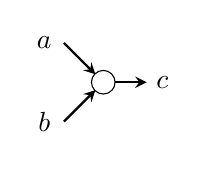
\begin{tikzpicture}[>=stealth]
\draw[->, thick] (2.25,0.5) -- (2.65,0.1);
\draw[->, thick] (2.25,-0.5) -- (2.65,-0.1);
\draw (2.75,0) ellipse (.15 and .15)[];
\draw[->,thick](2.9,0) -- (3.3,0);
           	   \node[] at (2.,0.5) {$a$};
           	              	   \node[] at (2.,-0.5) {$b$};
           	              	              	              	   \node[] at (3.5,0) {$c$};
	\end{tikzpicture}
	%}
	 \newline
	   \begin{tabular}{|c|c|c|}
		\hline
			a &  b & c \\
		\hline
			$\times$ & $\times$  & $\times$\\ 
		\hline
			$\times$ & $\circ$  & $\bullet$\\ 
		\hline
			$\circ$ & $\times$  & $\bullet$\\ 
		\hline
			$\circ$ & $\circ$  & $\bullet$\\ 
		\hline
			$\bullet$ & $\bullet$  & $\circ$\\ 
		\hline
	\end{tabular}
	\end{minipage}
	
	 &
    %row 3 cel 2
          \begin{minipage}[t]{.3\linewidth}
          {\replicatorNodeNamedabc}
          \newline
      \begin{tabular}{|c|c|c|}
		\hline
			a &  b & c \\
		\hline
			$\times$ & $\times$  & $\times$\\ 
		\hline
			$\times$ & $\circ$  & $\bullet$\\ 
		\hline
			$\circ$ & $\times$  & $\bullet$\\ 
		\hline
			$\circ$ & $\circ$  & $\bullet$\\ 
		\hline
			$\bullet$ & $\bullet$  & $\circ$\\ 
		\hline
	\end{tabular}
	\end{minipage}&
    %row 3 cel 3
       \begin{minipage}[t]{.3\linewidth}
        {\routerNodeabc}
        \newline
        \centering    
        \begin{tabular}{|c|c|c|}
		\hline
			a &  b & c\\
		\hline
			$\times$ & $\times$  & $\times$\\ 
		\hline
			$\times$ & $\circ$  & $\bullet$\\ 
		\hline
			$\circ$ & $\times$  & $\bullet$\\ 
		\hline
			$\circ$ & $\circ$  & $\bullet$\\ 
		\hline
			$\bullet$ & $\bullet$  & $\circ$\\ 
		\hline
	\end{tabular}
				         \vspace{.1cm}
    \end{minipage}    
 \\ \hline
\end{longtable}


\begin{BehExample}
Figure \ref{fig:prioex1} depicts a Reo network with a Priority sync. Here, we compute the priority coloring table of the network.

\begin{figure}[h]
\centering
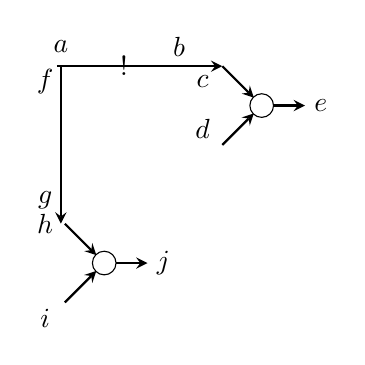
\begin{tikzpicture}[>=stealth]
\draw[->, thick] (2.25,0.5) -- (2.65,0.1);
\draw[->, thick] (2.25,-0.5) -- (2.65,-0.1);
\draw (2.75,0) ellipse (.15 and .15)[];
\draw[->,thick](2.9,0) -- (3.3,0);
           	   \node[] at (2.,0.3) {$c$};
           	              	   \node[] at (2.,-0.3) {$d$};
       	              	              	              	   \node[] at (3.5,0) {$e$};
       	              	              	              	   %%
       	              	              	              	    \node[] at (1.7,.75) {$b$};
       	              	              	              	        \node[] at (.2,.75) {$a$};
       	              	              	              	        \draw[->, thick] (.15,.5) -- (2.25,.5);
       	              	              	              	        \node[] at (1,.5) {$!$};
       	              	              	              	        %%
       	              	              	              	         \node[] at (0,.3) {$f$};
       	              	              	              	        \node[] at (0,-1.2) {$g$};
       	              	              	              	        \draw[->, thick] (.2,.5) -- (.2,-1.5);
       	              	              	              	        %%
       	              	              	              	        \draw[->, thick] (.25,-1.5) -- (.65,-1.9);
\draw[->, thick] (.25,-0.5-2) -- (.65,-0.1-2);
\draw (.75,-2) ellipse (.15 and .15)[];
\draw[->,thick](.9,-2) -- (1.3,-2);
           	   \node[] at (0,-1.5) {$h$};
           	              	   \node[] at (0,-2.7) {$i$};
       	              	              	              	   \node[] at (1.5,-2) {$j$};
\end{tikzpicture}
\caption{Example of Reo network with priority}
\label{fig:prioex1}
\end{figure}
\end{BehExample}

\noindent
\begin{minipage}{\linewidth}
\hfill
    \begin{minipage}[t]{.99\linewidth}
    \centering    
          \begin{tabular}{|c|c|c|c|c|}
		\hline
			a & b & c &  d & e \\
		\hline
$\bullet$ &$\bullet$ &$\circ$ &$\circ$ &$\bullet$  \\ \hline$\bullet$ &$\bullet$ &$\circ$ &$\times$ &$\bullet$  \\ \hline$\bullet$ &$\bullet$ &$\bullet$ &$\bullet$ &$\circ$  \\   \hline \end{tabular}      %  \captionof{sub figure}[short]{Connecting Sync channel and Join node}
       \label{twoooooo}
    \end{minipage}    
    \captionof{table}{Priority Coloring for joining $PrioritySync_{a,b}$ and $Join_{c,d,e}$}
    \label{mini:joinprioandsync}
\end{minipage}\hfill\null

\vspace{.5cm}

\noindent\begin{minipage}{\linewidth}
     \hfill
    \begin{minipage}[t]{.99\linewidth}
    \centering    
          \begin{tabular}{|c|c|c|c|c|c|c|}
		\hline
			a & b &c & d &e &  f & g \\
		\hline
			$\bullet$ &$\bullet$ &$\circ$ &$\circ$ &$\bullet$ &$\circ$ &$\bullet$  \\ \hline$\bullet$ &$\bullet$ &$\circ$ &$\circ$ &$\bullet$ &$\bullet$ &$\circ$  \\ \hline$\bullet$ &$\bullet$ &$\circ$ &$\times$ &$\bullet$ &$\circ$ &$\bullet$  \\ \hline$\bullet$ &$\bullet$ &$\circ$ &$\times$ &$\bullet$ &$\bullet$ &$\circ$  \\ \hline$\bullet$ &$\bullet$ &$\bullet$ &$\bullet$ &$\circ$ &$\circ$ &$\bullet$  \\ \hline$\bullet$ &$\bullet$ &$\bullet$ &$\bullet$ &$\circ$ &$\bullet$ &$\circ$  \\   \hline \end{tabular}
	
    %    \captionof{sub figure}[short]{join node and sync}
       \label{twoooooo}
    \end{minipage}    
    \captionof{table}{Priority Coloring after joining $Sync_{f,g}$}
    \label{mini:join3things}
\end{minipage}\hfill\null
%We exclude the case of both giving in channel chera?

\begin{table}[H]
\centering
\begin{tabular}{|c|c|c|c|c|c|c|c|c|c|}
		\hline
			a & b &c & d &e &  f & g & h & i & j\\
 \hline
  $\bullet$ &$\bullet$ &$\circ$ &$\circ$ &$\bullet$ &$\circ$ &$\bullet$ &$\circ$ &$\circ$ &$\bullet$  \\ \hline$\bullet$ &$\bullet$ &$\circ$ &$\circ$ &$\bullet$ &$\circ$ &$\bullet$ &$\circ$ &$\times$ &$\bullet$  \\ \hline$\bullet$ &$\bullet$ &$\circ$ &$\circ$ &$\bullet$ &$\circ$ &$\bullet$ &$\bullet$ &$\bullet$ &$\circ$  \\ \hline$\bullet$ &$\bullet$ &$\circ$ &$\circ$ &$\bullet$ &$\bullet$ &$\circ$ &$\bullet$ &$\bullet$ &$\circ$  \\ \hline$\bullet$ &$\bullet$ &$\circ$ &$\times$ &$\bullet$ &$\circ$ &$\bullet$ &$\circ$ &$\circ$ &$\bullet$  \\ \hline$\bullet$ &$\bullet$ &$\circ$ &$\times$ &$\bullet$ &$\circ$ &$\bullet$ &$\circ$ &$\times$ &$\bullet$  \\ \hline$\bullet$ &$\bullet$ &$\circ$ &$\times$ &$\bullet$ &$\circ$ &$\bullet$ &$\bullet$ &$\bullet$ &$\circ$  \\ \hline$\bullet$ &$\bullet$ &$\circ$ &$\times$ &$\bullet$ &$\bullet$ &$\circ$ &$\bullet$ &$\bullet$ &$\circ$  \\ \hline$\bullet$ &$\bullet$ &$\bullet$ &$\bullet$ &$\circ$ &$\circ$ &$\bullet$ &$\circ$ &$\circ$ &$\bullet$  \\ \hline$\bullet$ &$\bullet$ &$\bullet$ &$\bullet$ &$\circ$ &$\circ$ &$\bullet$ &$\circ$ &$\times$ &$\bullet$  \\ \hline$\bullet$ &$\bullet$ &$\bullet$ &$\bullet$ &$\circ$ &$\circ$ &$\bullet$ &$\bullet$ &$\bullet$ &$\circ$  \\ \hline$\bullet$ &$\bullet$ &$\bullet$ &$\bullet$ &$\circ$ &$\bullet$ &$\circ$ &$\bullet$ &$\bullet$ &$\circ$  \\   \hline \end{tabular}
\caption{Priority coloring table of the Reo network of Figure \ref{fig:prioex1}}
    \label{tab:mesalk}
\end{table}

Tables \ref{fig:prioex1} to \ref{tab:mesalk} illustrate construction of the coloring table for the Reo network of Figure \ref{fig:prioex1} step by step.

The $\circ$ color on the boundary nodes propagates potential priority imposed by parties that would join the current network.
However, to analyze the behavior of the network on the hand, we should exclude these rows. We refer to this operation as \emph{grounding}.

\begin{axiom}[Grounding Coloring Table]
Let $B \subset N$ be the set of boundary nodes in a Reo network. Grounding the coloring table of the network is done by ruling out the colors wherein a boundary node has the $\circ$ color.
\end{axiom}

\noindent
Table \ref{tab:mesalkg} is the result of grounding Table  \ref{tab:mesalk}. It indicates that the priority propagates from the \emph{PrioritySync}$_{a,b}$ channel propagates through the network.

% Later, we see effects of the propagated priority on non-deterministic choices of nodes $rep_{c,d,e}$ and $rep_{h,i,j}$. 

It illustrates that priority is propagated through the network and has affected all the node ends but $d$ and $i$. 

\begin{table}[H]
\centering
\begin{tabular}{|c|c|c|c|c|c|c|c|c|c|}
		\hline
			a & b &c & d &e &  f & g & h & i & j \\
 \hline
 $\bullet$ &$\bullet$ &$\circ$ &$\times$ &$\bullet$ &$\circ$ &$\bullet$ &$\circ$ &$\times$ &$\bullet$  \\  \hline \end{tabular}
   \caption{Grounded priority coloring table of the Reo network in Figure \ref{fig:prioex1}}
    \label{tab:mesalkg}
\end{table}


In chapter \ref{ch:bpmn} we mentioned that priority is essential for modeling transactions. Example \ref{ex:mesalbozorg} illustrates how we obtain the priority coloring table corresponding to a Reo transactional network.

\begin{BehExample}
\label{ex:mesalbozorg}
Figure \ref{fig:mesalebozorg} depicts the building block for implementing transactions in Reo. The \emph{FIFO}$_1$ represents a unit of work in a transaction, whose execution can be canceled or compensated. Since here we are merely interested in the effect of priority, we have omitted the compensation activity. %, which otherwise is shown in Figure  \ref{fig:mesalebozorgkamel}. 

\begin{figure}[h]
\includegraphics[width=8cm]{../08Priority/img/exampl2p}
\caption{A priority-sensitive Reo network}
\label{fig:mesalebozorg}
\end{figure}

%\begin{figure}[h]
%%\includegraphics[width=8cm]{../08Priority/img/mesalbozorg}
%\caption{????}
%\label{fig:mesalebozorgkamel}
%\end{figure}

%To avoid exploring the combinations of priority colors among nodes, which will be ruled out by grounding rule, we use grounding rule as soon as we deal with boundary nodes.

 Tables \ref{tab:j2}-\ref{tab:j11} illustrate the steps for computing the priority coloring table of the Figure \ref{fig:mesalebozorg}.  
%
%The grounded priority coloring of the boundary nodes $a$, $c$, and $g$ are presented in Tables \ref{tab:j1}, \ref{tab:j3}, and \ref{tab:j8}, respectively.

%\begin{table}
%\begin{tabular}{|c|c|c|}
%  \hline
%$a_1$ & $a_2$ & $a_3$ \\ 
%\hline
%$\times$ & $\times$ & $\times$ \\ 
%\hline
%$\bullet$ & $\circ$ & $\circ$ \\ 
%\hline
%$\bullet$ & $\circ$ & $\times$ \\ 
%\hline
%$\bullet$ & $\times$ & $\circ$ \\ 
%\hline
%\end{tabular}
%\caption{Grounded priority table of router $a$}
%\label{tab:j1}
%\end{table}

\begin{table}
\begin{tabular}{|c|c|c|c|c|}
  \hline
$a_1$ & $a_2$ & $a_3$ & $b_1$ & $b_2$ \\ 
\hline
$\times$ & $\times$ & $\times$ & $\times$ & $\times$ \\ 
\hline
$\times$ & $\times$ & $\times$ & $\times$ & $\circ$ \\ 
\hline
$\bullet$ & $\times$ & $\circ$ & $\times$ & $\times$ \\ 
\hline
$\bullet$ & $\times$ & $\circ$ & $\times$ & $\circ$ \\ 
\hline
\end{tabular}
\caption{Priority table obtained from joining $router_{a_1, a_2, a_3}$ and $FIFO_{b_1, b_2}$}
\label{tab:j2}
\end{table}
%By applying ground rule on node $c_2$, its priority coloring table is reduced to Table \ref{tab:j3}.
%\begin{table}
%\begin{tabular}{|c|c|c|}
%  \hline
%  $c_1$ & $c_2$ & $c_3$ \\
%  \hline
%  $\times$ & $\times$ & $\times$ \\
%  \hline
%  $\circ$ & $\bullet$ & $\bullet$ \\
%  \hline
%  $\bullet$ & $\times$ & $\circ$ \\
%  \hline
%\end{tabular}
%\caption{Grounded priority table of router $c$}
%\label{tab:j3}
%\end{table}

\begin{table}
\begin{tabular}{|c|c|c|c|c|c|c|c|}
  \hline
 $a_1$ & $a_2$ & $a_3$ & $b_1$ & $b_2$ & $c_1$ & $c_2$ & $c_3$ \\ 
 \hline
 $\times$ & $\times$ & $\times$ & $\times$ & $\times$ & $\times$ & $\times$ & $\times$ \\ 
 \hline
 $\times$ & $\times$ & $\times$ & $\times$ & $\circ$ & $\bullet$ & $\circ$ & $\circ$ \\ 
 \hline
 $\times$ & $\times$ & $\times$ & $\times$ & $\circ$ & $\bullet$ & $\circ$ & $\times$ \\ 
 \hline
 $\times$ & $\times$ & $\times$ & $\times$ & $\circ$ & $\bullet$ & $\times$ & $\circ$ \\ 
 \hline
 $\bullet$ & $\times$ & $\circ$ & $\times$ & $\times$ & $\times$ & $\times$ & $\times$ \\ 
 \hline
 $\bullet$ & $\times$ & $\circ$ & $\times$ & $\circ$ & $\bullet$ & $\circ$ & $\circ$ \\ 
 \hline
 $\bullet$ & $\times$ & $\circ$ & $\times$ & $\circ$ & $\bullet$ & $\circ$ & $\times$ \\ 
 \hline
 $\bullet$ & $\times$ & $\circ$ & $\times$ & $\circ$ & $\bullet$ & $\times$ & $\circ$ \\ 
 \hline
\end{tabular}
\caption{Priority coloring table result of joining $Router_{c_1, c_2, c_3}$}
\label{tab:j4}
\end{table}

\begin{table}
\begin{tabular}{|c|c|c|c|c|c|c|c|c|c|}
  \hline
   $a_1$ & $a_2$ & $a_3$ & $b_1$ & $b_2$ & $c_1$ & $c_2$ & $c_3$ & $d_1$ & $d_2$ \\ 
  \hline
  $\times$ & $\times$ & $\times$ & $\times$ & $\circ$ & $\bullet$ & $\circ$ & $\circ$ & $\bullet$ & $\bullet$ \\ 
  \hline
  $\times$ & $\times$ & $\times$ & $\times$ & $\circ$ & $\bullet$ & $\times$ & $\circ$ & $\bullet$ & $\bullet$ \\ 
  \hline
  $\bullet$ & $\times$ & $\circ$ & $\times$ & $\circ$ & $\bullet$ & $\circ$ & $\circ$ & $\bullet$ & $\bullet$ \\ 
  \hline
  $\bullet$ & $\times$ & $\circ$ & $\times$ & $\circ$ & $\bullet$ & $\times$ & $\circ$ & $\bullet$ & $\bullet$ \\ 
  \hline
\end{tabular}
\caption{Priority coloring table result of joining $PrioritySync_{d_1, d_2}$}
\label{tab:j5}
\end{table}

\begin{table}
\begin{tabular}{|c|c|c|c|c|c|c|c|c|c|c|c|}
  \hline
$a_1$ & $a_2$ & $a_3$ & $b_1$ & $b_2$ & $c_1$ & $c_2$ & $c_3$ & $d_1$ & $d_2$ & $e_1$ & $e_2$ \\ 
\hline
$\times$ & $\times$ & $\times$ & $\times$ & $\circ$ & $\bullet$ & $\circ$ & $\circ$ & $\bullet$ & $\bullet$ & $\circ$ & $\bullet$ \\ 
\hline
$\times$ & $\times$ & $\times$ & $\times$ & $\circ$ & $\bullet$ & $\circ$ & $\circ$ & $\bullet$ & $\bullet$ & $\bullet$ & $\circ$ \\ 
\hline
$\times$ & $\times$ & $\times$ & $\times$ & $\circ$ & $\bullet$ & $\times$ & $\circ$ & $\bullet$ & $\bullet$ & $\circ$ & $\bullet$ \\ 
\hline
$\times$ & $\times$ & $\times$ & $\times$ & $\circ$ & $\bullet$ & $\times$ & $\circ$ & $\bullet$ & $\bullet$ & $\bullet$ & $\circ$ \\ 
\hline
$\bullet$ & $\times$ & $\circ$ & $\times$ & $\circ$ & $\bullet$ & $\circ$ & $\circ$ & $\bullet$ & $\bullet$ & $\circ$ & $\bullet$ \\ 
\hline
$\bullet$ & $\times$ & $\circ$ & $\times$ & $\circ$ & $\bullet$ & $\circ$ & $\circ$ & $\bullet$ & $\bullet$ & $\bullet$ & $\circ$ \\ 
\hline
$\bullet$ & $\times$ & $\circ$ & $\times$ & $\circ$ & $\bullet$ & $\times$ & $\circ$ & $\bullet$ & $\bullet$ & $\circ$ & $\bullet$ \\ 
\hline
$\bullet$ & $\times$ & $\circ$ & $\times$ & $\circ$ & $\bullet$ & $\times$ & $\circ$ & $\bullet$ & $\bullet$ & $\bullet$ & $\circ$ \\ 
\hline
\end{tabular}
\caption{Priority coloring table result of joining $SyncDrain_{e_1, e_2}$}
\label{tab:j6}
\end{table}

\begin{table}
{\setlength\tabcolsep{3.25pt}
\noindent
\begin{tabular}{|c|c|c|c|c|c|c|c|c|c|c|c|c|c|c|}
  \hline
 $a_1$ & $a_2$ & $a_3$ & $b_1$ & $b_2$ & $c_1$ & $c_2$ & $c_3$ & $d_1$ & $d_2$ & $e_1$ & $e_2$ & $f_2$ & $f_1$ & $f_3$ \\ 
\hline
$\times$ & $\times$ & $\times$ & $\times$ & $\circ$ & $\bullet$ & $\circ$ & $\circ$ & $\bullet$ & $\bullet$ & $\circ$ & $\bullet$ & $\bullet$ & $\circ$ & $\circ$ \\ 
\hline
$\times$ & $\times$ & $\times$ & $\times$ & $\circ$ & $\bullet$ & $\circ$ & $\circ$ & $\bullet$ & $\bullet$ & $\circ$ & $\bullet$ & $\bullet$ & $\circ$ & $\times$ \\ 
\hline
$\times$ & $\times$ & $\times$ & $\times$ & $\circ$ & $\bullet$ & $\times$ & $\circ$ & $\bullet$ & $\bullet$ & $\circ$ & $\bullet$ & $\bullet$ & $\circ$ & $\circ$ \\ 
\hline
$\times$ & $\times$ & $\times$ & $\times$ & $\circ$ & $\bullet$ & $\times$ & $\circ$ & $\bullet$ & $\bullet$ & $\circ$ & $\bullet$ & $\bullet$ & $\circ$ & $\times$ \\ 
\hline
$\bullet$ & $\times$ & $\circ$ & $\times$ & $\circ$ & $\bullet$ & $\circ$ & $\circ$ & $\bullet$ & $\bullet$ & $\circ$ & $\bullet$ & $\bullet$ & $\circ$ & $\circ$ \\ 
\hline
$\bullet$ & $\times$ & $\circ$ & $\times$ & $\circ$ & $\bullet$ & $\circ$ & $\circ$ & $\bullet$ & $\bullet$ & $\circ$ & $\bullet$ & $\bullet$ & $\circ$ & $\times$ \\ 
\hline
$\bullet$ & $\times$ & $\circ$ & $\times$ & $\circ$ & $\bullet$ & $\times$ & $\circ$ & $\bullet$ & $\bullet$ & $\circ$ & $\bullet$ & $\bullet$ & $\circ$ & $\circ$ \\ 
\hline
$\bullet$ & $\times$ & $\circ$ & $\times$ & $\circ$ & $\bullet$ & $\times$ & $\circ$ & $\bullet$ & $\bullet$ & $\circ$ & $\bullet$ & $\bullet$ & $\circ$ & $\times$ \\ 
\hline
\end{tabular}
}
\caption{Priority coloring table result of joining $Router_{f_1, f_2, f_3}$}
\label{tab:j7}
\end{table}
%
%\begin{table}
%\begin{tabular}{|c|c|}
%  \hline
%  $g_1$ & $g_2$ \\
%  \hline
%  $\times$ & $\times$ \\
%  \hline
%  $\circ$ & $\bullet$ \\
%  \hline
%  $\circ$ & $\times$??? \\
%  \hline
%\end{tabular}
%\caption{Grounded priority table of router $g$}
%\label{tab:j8}
%\end{table}

\begin{table}
{\setlength\tabcolsep{3.25pt}
\noindent
\begin{tabular}{|c|c|c|c|c|c|c|c|c|c|c|c|c|c|c|c|c|}
  \hline
 $a_1$ & $a_2$ & $a_3$ & $b_1$ & $b_2$ & $c_1$ & $c_2$ & $c_3$ & $d_1$ & $d_2$ & $e_1$ & $e_2$ & $f_2$ & $f_1$ & $f_3$ & $g_2$ & $g_1$ \\ 
\hline
$\times$ & $\times$ & $\times$ & $\times$ & $\circ$ & $\bullet$ & $\circ$ & $\circ$ & $\bullet$ & $\bullet$ & $\circ$ & $\bullet$ & $\bullet$ & $\circ$ & $\circ$ & $\circ$ & $\bullet$ \\ 
\hline
$\times$ & $\times$ & $\times$ & $\times$ & $\circ$ & $\bullet$ & $\circ$ & $\circ$ & $\bullet$ & $\bullet$ & $\circ$ & $\bullet$ & $\bullet$ & $\circ$ & $\circ$ & $\bullet$ & $\circ$ \\ 
\hline
$\times$ & $\times$ & $\times$ & $\times$ & $\circ$ & $\bullet$ & $\circ$ & $\circ$ & $\bullet$ & $\bullet$ & $\circ$ & $\bullet$ & $\bullet$ & $\circ$ & $\times$ & $\circ$ & $\bullet$ \\ 
\hline
$\times$ & $\times$ & $\times$ & $\times$ & $\circ$ & $\bullet$ & $\circ$ & $\circ$ & $\bullet$ & $\bullet$ & $\circ$ & $\bullet$ & $\bullet$ & $\circ$ & $\times$ & $\bullet$ & $\circ$ \\ 
\hline
$\times$ & $\times$ & $\times$ & $\times$ & $\circ$ & $\bullet$ & $\times$ & $\circ$ & $\bullet$ & $\bullet$ & $\circ$ & $\bullet$ & $\bullet$ & $\circ$ & $\circ$ & $\circ$ & $\bullet$ \\ 
\hline
$\times$ & $\times$ & $\times$ & $\times$ & $\circ$ & $\bullet$ & $\times$ & $\circ$ & $\bullet$ & $\bullet$ & $\circ$ & $\bullet$ & $\bullet$ & $\circ$ & $\circ$ & $\bullet$ & $\circ$ \\ 
\hline
$\times$ & $\times$ & $\times$ & $\times$ & $\circ$ & $\bullet$ & $\times$ & $\circ$ & $\bullet$ & $\bullet$ & $\circ$ & $\bullet$ & $\bullet$ & $\circ$ & $\times$ & $\circ$ & $\bullet$ \\ 
\hline
$\times$ & $\times$ & $\times$ & $\times$ & $\circ$ & $\bullet$ & $\times$ & $\circ$ & $\bullet$ & $\bullet$ & $\circ$ & $\bullet$ & $\bullet$ & $\circ$ & $\times$ & $\bullet$ & $\circ$ \\ 
\hline
$\bullet$ & $\times$ & $\circ$ & $\times$ & $\circ$ & $\bullet$ & $\circ$ & $\circ$ & $\bullet$ & $\bullet$ & $\circ$ & $\bullet$ & $\bullet$ & $\circ$ & $\circ$ & $\circ$ & $\bullet$ \\ 
\hline
$\bullet$ & $\times$ & $\circ$ & $\times$ & $\circ$ & $\bullet$ & $\circ$ & $\circ$ & $\bullet$ & $\bullet$ & $\circ$ & $\bullet$ & $\bullet$ & $\circ$ & $\circ$ & $\bullet$ & $\circ$ \\ 
\hline
$\bullet$ & $\times$ & $\circ$ & $\times$ & $\circ$ & $\bullet$ & $\circ$ & $\circ$ & $\bullet$ & $\bullet$ & $\circ$ & $\bullet$ & $\bullet$ & $\circ$ & $\times$ & $\circ$ & $\bullet$ \\ 
\hline
$\bullet$ & $\times$ & $\circ$ & $\times$ & $\circ$ & $\bullet$ & $\circ$ & $\circ$ & $\bullet$ & $\bullet$ & $\circ$ & $\bullet$ & $\bullet$ & $\circ$ & $\times$ & $\bullet$ & $\circ$ \\ 
\hline
$\bullet$ & $\times$ & $\circ$ & $\times$ & $\circ$ & $\bullet$ & $\times$ & $\circ$ & $\bullet$ & $\bullet$ & $\circ$ & $\bullet$ & $\bullet$ & $\circ$ & $\circ$ & $\circ$ & $\bullet$ \\ 
\hline
$\bullet$ & $\times$ & $\circ$ & $\times$ & $\circ$ & $\bullet$ & $\times$ & $\circ$ & $\bullet$ & $\bullet$ & $\circ$ & $\bullet$ & $\bullet$ & $\circ$ & $\circ$ & $\bullet$ & $\circ$ \\ 
\hline
$\bullet$ & $\times$ & $\circ$ & $\times$ & $\circ$ & $\bullet$ & $\times$ & $\circ$ & $\bullet$ & $\bullet$ & $\circ$ & $\bullet$ & $\bullet$ & $\circ$ & $\times$ & $\circ$ & $\bullet$ \\ 
\hline
$\bullet$ & $\times$ & $\circ$ & $\times$ & $\circ$ & $\bullet$ & $\times$ & $\circ$ & $\bullet$ & $\bullet$ & $\circ$ & $\bullet$ & $\bullet$ & $\circ$ & $\times$ & $\bullet$ & $\circ$ \\ 
\hline
\end{tabular}
}
\caption{Priority coloring table result of $LossySync_{g_1, g_2}$}
\label{tab:j9}
\end{table}

\begin{table}
{\setlength\tabcolsep{3.25pt}
\noindent
\begin{tabular}{|c|c|c|c|c|c|c|c|c|c|c|c|c|c|c|c|c|c|c|}
  \hline
   $a_1$ & $a_2$ & $a_3$ & $b_1$ & $b_2$ & $c_1$ & $c_2$ & $c_3$ & $d_1$ & $d_2$ & $e_1$ & $e_2$ & $f_2$ & $f_1$ & $f_3$ & $g_2$ & $g_1$ & $h_1$ & $h_2$ \\ 
  \hline
  $\times$ & $\times$ & $\times$ & $\times$ & $\circ$ & $\bullet$ & $\circ$ & $\circ$ & $\bullet$ & $\bullet$ & $\circ$ & $\bullet$ & $\bullet$ & $\circ$ & $\circ$ & $\circ$ & $\bullet$ & $\bullet$ & $\circ$ \\ 
  \hline
  $\times$ & $\times$ & $\times$ & $\times$ & $\circ$ & $\bullet$ & $\circ$ & $\circ$ & $\bullet$ & $\bullet$ & $\circ$ & $\bullet$ & $\bullet$ & $\circ$ & $\circ$ & $\bullet$ & $\circ$ & $\bullet$ & $\circ$ \\ 
  \hline
  $\times$ & $\times$ & $\times$ & $\times$ & $\circ$ & $\bullet$ & $\circ$ & $\circ$ & $\bullet$ & $\bullet$ & $\circ$ & $\bullet$ & $\bullet$ & $\circ$ & $\times$ & $\circ$ & $\bullet$ & $\times$ & $\times$ \\ 
  \hline
  $\times$ & $\times$ & $\times$ & $\times$ & $\circ$ & $\bullet$ & $\circ$ & $\circ$ & $\bullet$ & $\bullet$ & $\circ$ & $\bullet$ & $\bullet$ & $\circ$ & $\times$ & $\bullet$ & $\circ$ & $\times$ & $\times$ \\ 
  \hline
  $\times$ & $\times$ & $\times$ & $\times$ & $\circ$ & $\bullet$ & $\times$ & $\circ$ & $\bullet$ & $\bullet$ & $\circ$ & $\bullet$ & $\bullet$ & $\circ$ & $\circ$ & $\circ$ & $\bullet$ & $\bullet$ & $\circ$ \\ 
  \hline
  $\times$ & $\times$ & $\times$ & $\times$ & $\circ$ & $\bullet$ & $\times$ & $\circ$ & $\bullet$ & $\bullet$ & $\circ$ & $\bullet$ & $\bullet$ & $\circ$ & $\circ$ & $\bullet$ & $\circ$ & $\bullet$ & $\circ$ \\ 
  \hline
  $\times$ & $\times$ & $\times$ & $\times$ & $\circ$ & $\bullet$ & $\times$ & $\circ$ & $\bullet$ & $\bullet$ & $\circ$ & $\bullet$ & $\bullet$ & $\circ$ & $\times$ & $\circ$ & $\bullet$ & $\times$ & $\times$ \\ 
  \hline
  $\times$ & $\times$ & $\times$ & $\times$ & $\circ$ & $\bullet$ & $\times$ & $\circ$ & $\bullet$ & $\bullet$ & $\circ$ & $\bullet$ & $\bullet$ & $\circ$ & $\times$ & $\bullet$ & $\circ$ & $\times$ & $\times$ \\ 
  \hline
  $\bullet$ & $\times$ & $\circ$ & $\times$ & $\circ$ & $\bullet$ & $\circ$ & $\circ$ & $\bullet$ & $\bullet$ & $\circ$ & $\bullet$ & $\bullet$ & $\circ$ & $\circ$ & $\circ$ & $\bullet$ & $\bullet$ & $\circ$ \\ 
  \hline
  $\bullet$ & $\times$ & $\circ$ & $\times$ & $\circ$ & $\bullet$ & $\circ$ & $\circ$ & $\bullet$ & $\bullet$ & $\circ$ & $\bullet$ & $\bullet$ & $\circ$ & $\circ$ & $\bullet$ & $\circ$ & $\bullet$ & $\circ$ \\ 
  \hline
  $\bullet$ & $\times$ & $\circ$ & $\times$ & $\circ$ & $\bullet$ & $\circ$ & $\circ$ & $\bullet$ & $\bullet$ & $\circ$ & $\bullet$ & $\bullet$ & $\circ$ & $\times$ & $\circ$ & $\bullet$ & $\times$ & $\times$ \\ 
  \hline
  $\bullet$ & $\times$ & $\circ$ & $\times$ & $\circ$ & $\bullet$ & $\circ$ & $\circ$ & $\bullet$ & $\bullet$ & $\circ$ & $\bullet$ & $\bullet$ & $\circ$ & $\times$ & $\bullet$ & $\circ$ & $\times$ & $\times$ \\ 
  \hline
  $\bullet$ & $\times$ & $\circ$ & $\times$ & $\circ$ & $\bullet$ & $\times$ & $\circ$ & $\bullet$ & $\bullet$ & $\circ$ & $\bullet$ & $\bullet$ & $\circ$ & $\circ$ & $\circ$ & $\bullet$ & $\bullet$ & $\circ$ \\ 
  \hline
  $\bullet$ & $\times$ & $\circ$ & $\times$ & $\circ$ & $\bullet$ & $\times$ & $\circ$ & $\bullet$ & $\bullet$ & $\circ$ & $\bullet$ & $\bullet$ & $\circ$ & $\circ$ & $\bullet$ & $\circ$ & $\bullet$ & $\circ$ \\ 
  \hline
  $\bullet$ & $\times$ & $\circ$ & $\times$ & $\circ$ & $\bullet$ & $\times$ & $\circ$ & $\bullet$ & $\bullet$ & $\circ$ & $\bullet$ & $\bullet$ & $\circ$ & $\times$ & $\circ$ & $\bullet$ & $\times$ & $\times$ \\ 
  \hline
  $\bullet$ & $\times$ & $\circ$ & $\times$ & $\circ$ & $\bullet$ & $\times$ & $\circ$ & $\bullet$ & $\bullet$ & $\circ$ & $\bullet$ & $\bullet$ & $\circ$ & $\times$ & $\bullet$ & $\circ$ & $\times$ & $\times$ \\ 
  \hline
\end{tabular}
}
\caption{Priority coloring table result of $SyncDrain_{h_1, h_2}$}
\label{tab:j10}
\end{table}

\begin{table}
{\setlength\tabcolsep{3.25pt}
\noindent
\begin{tabular}{|c|c|c|c|c|c|c|c|c|c|c|c|c|c|c|c|c|c|c|c|c|}
  \hline
$a_1$ & $a_2$ & $a_3$ & $b_1$ & $b_2$ & $c_1$ & $c_2$ & $c_3$ & $d_1$ & $d_2$ & $e_1$ & $e_2$ & $f_2$ & $f_1$ & $f_3$ & $g_2$ & $g_1$ & $h_1$ & $h_2$ & $i_2$ & $i_1$ \\ 
\hline
$\times$ & $\times$ & $\times$ & $\times$ & $\circ$ & $\bullet$ & $\circ$ & $\circ$ & $\bullet$ & $\bullet$ & $\circ$ & $\bullet$ & $\bullet$ & $\circ$ & $\circ$ & $\circ$ & $\bullet$ & $\bullet$ & $\circ$ & $\bullet$ & $\bullet$ \\ 
\hline
$\times$ & $\times$ & $\times$ & $\times$ & $\circ$ & $\bullet$ & $\circ$ & $\circ$ & $\bullet$ & $\bullet$ & $\circ$ & $\bullet$ & $\bullet$ & $\circ$ & $\circ$ & $\bullet$ & $\circ$ & $\bullet$ & $\circ$ & $\bullet$ & $\bullet$ \\ 
\hline
$\times$ & $\times$ & $\times$ & $\times$ & $\circ$ & $\bullet$ & $\times$ & $\circ$ & $\bullet$ & $\bullet$ & $\circ$ & $\bullet$ & $\bullet$ & $\circ$ & $\circ$ & $\circ$ & $\bullet$ & $\bullet$ & $\circ$ & $\bullet$ & $\bullet$ \\ 
\hline
$\times$ & $\times$ & $\times$ & $\times$ & $\circ$ & $\bullet$ & $\times$ & $\circ$ & $\bullet$ & $\bullet$ & $\circ$ & $\bullet$ & $\bullet$ & $\circ$ & $\circ$ & $\bullet$ & $\circ$ & $\bullet$ & $\circ$ & $\bullet$ & $\bullet$ \\ 
\hline
$\bullet$ & $\times$ & $\circ$ & $\times$ & $\circ$ & $\bullet$ & $\circ$ & $\circ$ & $\bullet$ & $\bullet$ & $\circ$ & $\bullet$ & $\bullet$ & $\circ$ & $\circ$ & $\circ$ & $\bullet$ & $\bullet$ & $\circ$ & $\bullet$ & $\bullet$ \\ 
\hline
$\bullet$ & $\times$ & $\circ$ & $\times$ & $\circ$ & $\bullet$ & $\circ$ & $\circ$ & $\bullet$ & $\bullet$ & $\circ$ & $\bullet$ & $\bullet$ & $\circ$ & $\circ$ & $\bullet$ & $\circ$ & $\bullet$ & $\circ$ & $\bullet$ & $\bullet$ \\ 
\hline
$\bullet$ & $\times$ & $\circ$ & $\times$ & $\circ$ & $\bullet$ & $\times$ & $\circ$ & $\bullet$ & $\bullet$ & $\circ$ & $\bullet$ & $\bullet$ & $\circ$ & $\circ$ & $\circ$ & $\bullet$ & $\bullet$ & $\circ$ & $\bullet$ & $\bullet$ \\ 
\hline
$\bullet$ & $\times$ & $\circ$ & $\times$ & $\circ$ & $\bullet$ & $\times$ & $\circ$ & $\bullet$ & $\bullet$ & $\circ$ & $\bullet$ & $\bullet$ & $\circ$ & $\circ$ & $\bullet$ & $\circ$ & $\bullet$ & $\circ$ & $\bullet$ & $\bullet$ \\ 
\hline
\end{tabular}
}
\caption{Priority coloring table of Figure \ref{fig:mesalebozorg} result of $PrioritySync_{i_1, i_2}$}
\label{tab:j11}
\end{table}

Table \ref{tab:j12} illustrates that the priority has been propagated through the network. It shows that all the nodes except $a_2$, $b_1$, and $c_2$ have  priority. 

\begin{table}
{\setlength\tabcolsep{3.25pt}
\noindent
\begin{tabular}{|c|c|c|c|c|c|c|c|c|c|c|c|c|c|c|c|c|c|c|c|c|}
  \hline
$a_1$ & $a_2$ & $a_3$ & $b_1$ & $b_2$ & $c_1$ & $c_2$ & $c_3$ & $d_1$ & $d_2$ & $e_1$ & $e_2$ & $f_2$ & $f_1$ & $f_3$ & $g_2$ & $g_1$ & $h_1$ & $h_2$ & $i_2$ & $i_1$ \\ 
\hline
$\bullet$ & $\times$ & $\circ$ & $\times$ & $\circ$ & $\bullet$ & $\times$ & $\circ$ & $\bullet$ & $\bullet$ & $\circ$ & $\bullet$ & $\bullet$ & $\circ$ & $\circ$ & $\bullet$ & $\circ$ & $\bullet$ & $\circ$ & $\bullet$ & $\bullet$ \\ 
\hline
\end{tabular}
}
\caption{Grounded priority table of router $c$}
\label{tab:j12}
\end{table}
\end{BehExample}



\begin{BehExample}
	\label{ex:example3}
	Our last example in this chapter illustrates how blocking of priority is handled in our priority coloring model.
	
	\tikzstyle{block} = [circle, minimum width=2mm, draw, text centered]
	\tikzstyle{line} = [draw, ->]
	
	\[ \begin{tikzpicture}[node distance=2cm]
	\node [] (a) {};
	\node [block, right of = a] (b) {};
	\node [block, right of = b] (c) {};
	\node [below of = b, node distance=.5cm] (d) {};
	\node [below of = c] (e) {m};
	\node [right of = c, node distance=.7cm] (f) {k};
	
	\node [label={[label distance=.8cm]1:!}]{};
	\node [label={[label distance=2.7cm]1:)}]{};
	\node [label={[label distance=3.7cm]-13:--.}]{};
	\node [label={[label distance=.1cm]3:a}]{};
	\node [label={[label distance=1cm]3:b}]{};
	\node [label={[label distance=1.3cm]-8:d}]{};
	\node [label={[label distance=1.3cm]3:c}]{};
	\node [label={[label distance=2.2cm]-3:f}]{};
	\node [label={[label distance=3.1cm]2:g}]{};
	%\node [label={[label distance=3.3cm]4:h}]{};
	\node [label={[label distance=2.1cm]4:e}]{}; 
	%\node [label={[label distance=3.3cm]-86:k}]{};
	\node [label={[label distance=3.5cm]4:i}]{};
	\node [label={[label distance=3.5cm]-3:j}]{};
	\node [label={[label distance=3.9cm]-5:l}]{};
	
	\path [line] (a) -- (b);
	\path [line] (d) -- (b);
	\path [line] (b) -- (c);
	\path [line] (e) -- (c);
	\path [line] (c) -- (f);
	\end{tikzpicture} \]


%
%
%\begin{table}
%	%	{\setlength\tabcolsep{3.25pt}
%	\noindent
%	\begin{tabular}{|c|c|}
%		\hline
%		a&b\\ 
%		\hline
%		$\bullet$ & $\bullet$ \\ 
%		\hline
%	\end{tabular}
%\end{table}

\begin{table}
	%	{\setlength\tabcolsep{3.25pt}
	\noindent
	\begin{tabular}{|c|c|c|c|c|}
		\hline
		a&b&c&d&e\\ 
		\hline
		$\bullet$ & $\bullet$ & $\circ$ & $\times$ & $\bullet$ \\ 
		\hline
		$\bullet$ & $\bullet$ & $\circ$ & $\circ$ & $\bullet$ \\ 
		\hline
		$\bullet$ & $\bullet$ & $\bullet$ & $\bullet$ & $\circ$ \\ 
		\hline
	\end{tabular}
\caption{Priority coloring table result of joining $PrioritySync_{a_1, b_2}$ and $Node_{c,d,e}$}
\label{tab:x1}
\end{table}

\begin{table}
	%	{\setlength\tabcolsep{3.25pt}
	\noindent
	\begin{tabular}{|c|c|c|c|c|c|c|}
		\hline
		a&b&c&d&e&f&g\\ 
		\hline
		$\bullet$ & $\bullet$ & $\circ$ & $\times$ & $\bullet$ & $\circ$ & $\times$ \\ 
		\hline
		$\bullet$ & $\bullet$ & $\circ$ & $\times$ & $\bullet$ & $\circ$ & $\circ$ \\ 
		\hline
		$\bullet$ & $\bullet$ & $\circ$ & $\circ$ & $\bullet$ & $\circ$ & $\times$ \\ 
		\hline
		$\bullet$ & $\bullet$ & $\circ$ & $\circ$ & $\bullet$ & $\circ$ & $\circ$ \\ 
		\hline
	\end{tabular}
\caption{Priority coloring table result of joining $BlockSourceSync_{f,g}$}
\label{tab:x2}
\end{table}


\begin{table}
	%	{\setlength\tabcolsep{3.25pt}
	\noindent
	\begin{tabular}{|c|c|c|c|c|c|c|c|c|c|}
		\hline
		a&b&c&d&e&f&g&i&j&k\\ 
		\hline
		$\bullet$ & $\bullet$ & $\circ$ & $\times$ & $\bullet$ & $\circ$ & $\times$ & $\times$ & $\times$ & $\times$ \\ 
		\hline
		$\bullet$ & $\bullet$ & $\circ$ & $\times$ & $\bullet$ & $\circ$ & $\times$ & $\times$ & $\circ$ & $\bullet$ \\ 
		\hline
		$\bullet$ & $\bullet$ & $\circ$ & $\times$ & $\bullet$ & $\circ$ & $\circ$ & $\bullet$ & $\bullet$ & $\circ$ \\ 
		\hline
		$\bullet$ & $\bullet$ & $\circ$ & $\circ$ & $\bullet$ & $\circ$ & $\times$ & $\times$ & $\times$ & $\times$ \\ 
		\hline
		$\bullet$ & $\bullet$ & $\circ$ & $\circ$ & $\bullet$ & $\circ$ & $\times$ & $\times$ & $\circ$ & $\bullet$ \\ 
		\hline
		$\bullet$ & $\bullet$ & $\circ$ & $\circ$ & $\bullet$ & $\circ$ & $\circ$ & $\bullet$ & $\bullet$ & $\circ$ \\ 
		\hline
	\end{tabular}
\caption{Priority coloring table result of joining $Node_{h,i,k}$}
\label{tab:x3}
\end{table} 

\begin{table}
	%	{\setlength\tabcolsep{3.25pt}
	\noindent
	\begin{tabular}{|c|c|c|c|c|c|c|c|c|c|c|c|}
		\hline
		a&b&c&d&e&f&g&i&j&k&l&m\\
		\hline
		$\bullet$ & $\bullet$ & $\circ$ & $\times$ & $\bullet$ & $\circ$ & $\times$ & $\times$ & $\circ$ & $\bullet$ & $\bullet$ & $\bullet$ \\ 
		\hline
		$\bullet$ & $\bullet$ & $\circ$ & $\times$ & $\bullet$ & $\circ$ & $\circ$ & $\bullet$ & $\bullet$ & $\circ$ & $\bullet$ & $\bullet$ \\ 
		\hline
		$\bullet$ & $\bullet$ & $\circ$ & $\circ$ & $\bullet$ & $\circ$ & $\times$ & $\times$ & $\circ$ & $\bullet$ & $\bullet$ & $\bullet$ \\ 
		\hline
		$\bullet$ & $\bullet$ & $\circ$ & $\circ$ & $\bullet$ & $\circ$ & $\circ$ & $\bullet$ & $\bullet$ & $\circ$ & $\bullet$ & $\bullet$ \\ 
		\hline
	\end{tabular}
\caption{Priority coloring table result of joining $PrioritySync_{j, l}$}
\label{tab:x4}
\end{table}

Table \ref{tab:x5} shows that the \emph{BlockSourceSync} has blocked propagation of priority to the $g$ and $i$ node ends. The node $d$ has no priority either. 

\begin{table}
	%	{\setlength\tabcolsep{3.25pt}
	\noindent
	\begin{tabular}{|c|c|c|c|c|c|c|c|c|c|c|c|}
		\hline	
		a&b&c&d&e&f&g&i&j&k&l&m\\
		\hline
		$\bullet$ & $\bullet$ & $\circ$ & $\times$ & $\bullet$ & $\circ$ & $\times$ & $\times$ & $\circ$ & $\bullet$ & $\bullet$ & $\bullet$ \\
		\hline
	\end{tabular}
	\caption{Grounded priority table for the Reo network in Example \ref{ex:example3}}
	\label{tab:x5}
\end{table}
\end{BehExample}

In order to propagate and consume priority as suggested by the introduced model, we need to update the constraints encoding the behavior of each primitives.  

\subsection{Encoding Priority Coloring Model in Constraints}
The presented priority model depicts the intuition for modeling propagation of priority in a Reo network. However, it lacks the data-flow and context information of the network. The priority propagation information needs to be incorporated in our constraint-based framework, presented in Chapter \ref{chapterCASM}.

The incorporation is two-folded: First, we express the priority propagation model in terms of constraints. Second, we modify the encodings of the Reo primitives  
in order for the priority assumptions to affect  non-deterministic choices between possible date-flows.

For the former, we extend the grammar of the constraints %that encode the behavior of a Reo network,
 presented in Section \ref{sec:ecsp}. %of Chapter \ref{chapterCASM}. 

%TODO
We introduce two Boolean variables $n^{!^\bullet}$ and $n^{!^\circ}$ to denote whether a node has imposed or innate priority, respectively. A node has priority iff at least one of these variables is $true$.

Recall from Chapter \ref{chapterCASM} the type of variables we use to describe the behavior of a Reo network as follows: 

%rephrase?
\begin{itemize}
 \item $\tilde{n}$ ranges over $\{ \top, \bot \}$ to show presence or absence of data-flow on the node $n$.
 \item $\hat{n}$ ranges over $\mathcal{D}$ to represent the data value passing through the node $n$.
 \item $\mathring{m}, \mathring{m}'$ range over $\{ \top, \bot \}$ to denote whether or not the state memory variable $m$ is defined in the source and the target states of the transition to which the encoded condition belongs, respectively.
 \item $\hat{m}, \hat{m}'$ range over $\mathcal{D}$ to represent the values of the state memory variable $m$ in, respectively, the source and the target states of the transition to which the encoded condition belongs.
 \item $p^\triangleright$ ranges over $\{ \top, \bot \}$ to indicate that the reason for lack of data-flow through the primitive end $p$ originates from the primitive to which $p$ belongs or the context (of this primitive), respectively.
\end{itemize}

The following is the updated grammar for a constraint $\Psi$ encoding the behavior of a Reo network, wherein
%\vspace*{.65cm}
%\noindent
$d \in \D$ is a constant, $\circledast \in \{+, -, \ast, /, \%, \tavan \}, $ and $p$ is  either of the form $n^c$ or $n^k$.

%\begin{table}[H]
\begin{tabular}{c c l l}
\centering
  & \\
  $t $&$::= $&$\hat{n}\ |\ \hat{m}\ |\ \hat{m}'\ |\ d\ |\ t \circledast \ d$ & (terms)\\
  $a $&$::=$&$ \tilde{n}\ |\ n^{!^\bullet}\ |\ n^{!^\circ}\ | \ p^\triangleright\ |\ \mathring{m}\ |\ \mathring{m}'\ |\ t=t\ |\ t<t $ & (atoms)\\
  $\Uppsi $&$::=$&$ \top \ | \ a\ |\ \neg \Uppsi \ | \ \Uppsi \wedge \ \Uppsi $ & (formulae)\\
  &
\end{tabular}
%\caption{Grammar of a constraint expressing the behavior of a Reo network}
%\label{tab:reoformulaupdated}
%\end{table}
%\vspace*{.2cm}

The followings shows how we encode the priority colors in constraints:

\begin{tabular}{c c c}
\centering
  $n = \bullet$ & $\Leftrightarrow$& $n^{!^\bullet} = \top$\\
  $n = \circ$  &$\Leftrightarrow$ &  $n^{!^\circ} = \top \ \wedge\  n^{!^\bullet} = \bot$\\
  $n = -$ &$\Leftrightarrow$ &$n^{!^\circ} = \bot \ \wedge\  n^{!^\bullet} = \bot$ \\
\end{tabular}



\noindent
The \emph{join} operator translates into the following axiom:

\begin{axiom}[Priority Join]\label{ax:joinprio}
When two Reo networks connect on the node $n$, where $c$ is a source end in one network and $k$ is a sink end in the other, the following constraint must hold:
$$(c^{!^\circ}\ \vee\ c^{!^\bullet} \Leftrightarrow k^{!^\circ}\ \vee\ k^{!^\bullet}) \ \wedge \ (c^{!^\circ}\ \wedge\ k^{!^\circ} \Leftrightarrow c^{!^\bullet}\ \vee\ k^{!^\bullet})$$
\end{axiom}

The \emph{priority join} axiom eliminates invalid priority coloring from the constraint results. It is straight-forward to see that the axiom is the encoding of the priority join operator in Definition \ref{def:priojoinoperator}.

%TODO
For priority to be able to affect the data-flow in a Reo network, two types of modification in the constraint encoding of the primitives are required: 

\begin{itemize}
\item All the primitives should propagate the priority information,
\item The primitives that perform non-deterministic choices between alternative data-flow should respect the propagated priority.
\end{itemize}

The former is achieved by constraining the variables that represent priority. For realizing the later, we need to exclude cases where a data-flow over a node with no priority is chosen over the data-flow over the prioritized node, while the prioritized node is ready to perform I/O actions. Axiom \ref{ax:chooserprio} carries out this requirement.

\begin{axiom}[Priority in Non-deterministic Choice]\label{ax:chooserprio}
Let $E$ be a set of node ends among them a Reo primitive chooses a node end for communication, non-deterministically.

We divide $E$ to two disjoint sets of the nodes, which have priority, described by $E_p=\{e | e \in E, e^{!^\circ}\ \wedge\ e^{!^\bullet}\}$, and those that do not have priority. The following predicate guarantees that a node with no priority has data-flow only if no prioritized node is ready to interact.

$$\bigvee_{x \in E_p} \tilde{x} \Rightarrow \bigwedge_{y \notin E_p} (\neg \tilde{y} \wedge y^\triangleright???) $$
\end{axiom}

Table \ref{tab:contextencodingprioadded2} depicts the constraint encoding of commonly-used Reo primitives.%rephrase?
\begin{center}
\begin{longtable}{|c|c|}%[H]
%\centering
%\scriptsize
%\begin{tabular}{|c|c|}
\caption{Priority Coloring of some commonly used Reo Primitives} \label{tab:contextencodingprioadded2}
\\
\hline
Channel & Constraints \\ 
\hline \vspace*{-.3cm} \\
 \tikz{%prio
          	   \node[point,label=left:$$] (A) {};
           	   \node[point,right of=A,label=right:$$, node distance=1cm] (B) {};
           	   \draw[sync] (A) -- (B);
           	   \node[] at (.5,0) {$!$};}
          & \parbox{.75\columnwidth}{$ \psi_{PrioritySync}(a, b) : (\tilde{a} \Leftrightarrow \tilde{b}) \wedge (\tilde{a} \Rightarrow (\hat{a}=\hat{b})) \wedge \neg(a^{c^\triangleright} \wedge b^{k^\triangleright})$ $\color{black} \wedge a^{!^\bullet} \wedge b^{!^\bullet}$} \\ %c^{!^\bullet}\ \vee\ k^{!^\bullet})
%BsSync  
	\tikz{%blok
          	   \node[point,label=left:$$] (A) {};
           	   \node[point,right of=A,label=right:$$, node distance=1cm] (B) {};
           	   \draw[sync] (A) -- (B);
           	   \node[] at (.5,0) {$)$};} & \parbox{.75\columnwidth}{$ \psi_{BlockSourceSync}(a, b) : (\tilde{a} \Leftrightarrow \tilde{b}) \wedge (\tilde{a} \Rightarrow (\hat{a}=\hat{b})) \wedge \neg(a^{^c\triangleright} \wedge b^{k^\triangleright})$ $\color{black} \wedge a^{!^\bullet} \wedge \neg b^{!^\bullet}$} \\
           	   %\\
%BkSync  
		\tikz{%blok
          	   \node[point,label=left:$$] (A) {};
           	   \node[point,right of=A,label=right:$$, node distance=1cm] (B) {};
           	   \draw[sync] (A) -- (B);
           	   \node[] at (.5,0) {$($};}	     & \parbox{.75\columnwidth}{$ \psi_{BlockSinkSync}(a, b) : (\tilde{a} \Leftrightarrow \tilde{b}) \wedge (\tilde{a} \Rightarrow (\hat{a}=\hat{b})) \wedge \neg(a^{c^\triangleright} \wedge b^{k^\triangleright})$ $\color{black} \wedge a^{!^\bullet} \wedge \neg b^{!^\bullet}$} \\
%BSync 2way 
		\tikz{%blok
          	   \node[point,label=left:$$] (A) {};
           	   \node[point,right of=A,label=right:$$, node distance=1cm] (B) {};
           	   \draw[sync] (A) -- (B);
           	   \node[] at (.5,0) {$)($};}	     & \parbox{.75\columnwidth}{$ \psi_{BlockSync}(a, b) : (\tilde{a} \Leftrightarrow \tilde{b}) \wedge (\tilde{a} \Rightarrow (\hat{a}=\hat{b})) \wedge \neg(a^{c^\triangleright} \wedge b^{k^\triangleright})$ $\color{black} \wedge a^{!^\bullet} \wedge \neg b^{!^\bullet}$} 
           	   \\
%sync
  {\sync}  & \parbox{.75\columnwidth}{$ \psi_{Sync}(a, b) : (\tilde{a} \Leftrightarrow \tilde{b}) \wedge (\tilde{a} \Rightarrow (\hat{a}=\hat{b})) \wedge \neg(a^{c^\triangleright} \wedge b^{k^\triangleright})$  
  $\color{black} \wedge \neg(a^{!^\bullet} \vee b^{!^\bullet} \vee a^{!^\circ} \vee b^{!^\circ}) \vee (a^{!^\bullet} \wedge \neg  b^{!^\bullet}  \wedge b^{!^\circ}) \vee (b^{!^\bullet} \wedge \neg b^{!^\bullet} \wedge b^{!^\circ} )$}  \\
	   %lossysync
	    {\lossysync} & \parbox{.75\columnwidth}{$\psi_{LossySync}(a, b) : \tilde{b} \Rightarrow \tilde{a} \wedge (\tilde{b} \Rightarrow (\hat{a}=\hat{b})) \wedge \neg a^{c^\triangleright} \wedge \neg \tilde{a} \Rightarrow b^{k^\triangleright}$} \\ 
           	   %syncdrain
{\syncdrain} & \parbox{.75\columnwidth}{$ \psi_{SyncDrain}(a_1, a_2) : \tilde{a}_1 \Leftrightarrow \tilde{a}_2 \wedge \neg(a_1^{c^\triangleright} \wedge a_2^{c^\triangleright})  \color{black} TODO: complete the rest$} \\
  %syncspout
{\syncspout}& \parbox{.75\columnwidth}{$ \psi_{SyncSpout}(k_1, k_2, \mathcal{P}_{k_1}, \mathcal{P}_{k_2}) : \tilde{k}_1 \Leftrightarrow \tilde{k}_2 \wedge \neg(k^{{\downarrow}}_1 \wedge k^{{\downarrow}}_2) \wedge \tilde{k}_1 \Rightarrow (\hat{k}_1 \in \mathcal{P}_{k_1}(\hat{k}_1)) \wedge \tilde{k}_2 \Rightarrow (\hat{k}_2 \in \mathcal{P}_{k_2}(\hat{k}_2)) $} \\
 {\asyncdrain} & \parbox{.75\columnwidth}{$ \psi_{AsyncDrain}(a_1, a_2) : \tilde{a}_1 \Rightarrow (\neg \tilde{a}_2 \wedge a_2^{c^\triangleright}) \wedge \tilde{a}_2 \Rightarrow (\neg \tilde{a}_1 \wedge a_1^{c^\triangleright})$} \\ 
 %asyncspout
 {\asyncspout} & \parbox{.75\columnwidth}{$ \psi_{AsyncSpout}(k_1, k_2) : \tilde{k}_1 \Rightarrow (k_{1}^{\downarrow} \neg \tilde{k}_2 \wedge \hat{k}_1 \in \mathcal{P}_{k_1}) \wedge \tilde{k}_2 \Rightarrow (k_{2}^{\downarrow} \wedge \neg \tilde{k}_1 \wedge \hat{k}_2 \in \mathcal{P}_{k_2})$} \\ %\\
%filter
  {\filterwithpredicate} & \parbox{.75\columnwidth}{$\psi_{Filter}(a, b, P) = (\tilde{b} \Rightarrow (\tilde{a} \wedge \hat{a} \in dom(P) \wedge P(\hat{a}))) \wedge (\tilde{b} \Rightarrow (\hat{a}=\hat{b})) \wedge %reason 
   (\neg \tilde{a} \Rightarrow (\neg a^{c^\triangleright} \Leftrightarrow b^{k^\triangleright})) \wedge
   (\tilde{a} \wedge \neg \tilde{b} \Rightarrow b^{k^\triangleright})$} \\ %\\
 {\transformerwithfunction} & \parbox{.75\columnwidth}{$ \psi_{Transformer}(a, b, f) = (\tilde{b} \Rightarrow (\tilde{a} \wedge \hat{a} \in  dom(f))) \wedge (\tilde{b} \Rightarrow (\hat{b}=f(\hat{a}))) \wedge %reason
 \neg (a^{c^\triangleright} \wedge b^{k^\triangleright})$} \\ 
 %fifo
 {\fifo} & \parbox{.75\columnwidth}{$ \psi_{FIFO_{1}}(a, b, m) : (\tilde{a} \Rightarrow (\neg \mathring{m} \wedge \mathring{m}' \wedge (\hat{m}'=\hat{a}))) \wedge (\tilde{b} \Rightarrow (\mathring{m} \wedge \neg \mathring{m}' \wedge (\hat{m}=\hat{b}))) \wedge ((\neg \tilde{a} \wedge \neg \tilde{b}) \Rightarrow (\mathring{m} \Leftrightarrow \mathring{m}' \wedge \mathring{m} \Rightarrow (\hat{m}=\hat{m}'))) \wedge %reasin
(\neg \mathring{m} \Rightarrow b^{k^\triangleright}) \wedge  (\mathring{m} \Rightarrow a^{c^\triangleright})
 $} \\
 %fullfifo\\
  {\fifofull} & \parbox{.75\columnwidth}{$ \psi_{FIFO_{1}}(a, b, m) :  (\tilde{a} \Rightarrow (\neg \mathring{m} \wedge \mathring{m}' \wedge (\hat{m}'=\hat{a}))) \wedge (\tilde{b} \Rightarrow (\mathring{m} \wedge \neg \mathring{m}' \wedge (\hat{m}=\hat{b}))) \wedge (\neg \tilde{a} \wedge \neg \tilde{b}) \Rightarrow (\mathring{m} \Leftrightarrow \mathring{m}' \wedge \mathring{m} \Rightarrow (\hat{m}=\hat{m}')) \wedge %reasin
(\neg \mathring{m} \Rightarrow b^{k^\triangleright}) \wedge  (\mathring{m} \Rightarrow a^{c^\triangleright})
 $} \\ 
 {\mergerNode} &  \parbox{.75\columnwidth}{$\psi_{Merger}(a_{0..i}, b) : \tilde{a}_i \Rightarrow \tilde{b} \wedge \tilde{a}_i \Rightarrow    (\hat{a_i}=\hat{b}) \wedge \neg \tilde{b} \Rightarrow ((\neg b^{k^\triangleright} \bigwedge_i a_i^{c^\triangleright}) \vee (b^{k^\triangleright} \wedge \neg a_i^{c^\triangleright} \bigwedge_{j, j!= i} a_j^{k^\triangleright}))$}\\ %\\   
 {\replicatorNode} & \parbox{.75\columnwidth}{$\psi_{Replicator}(a, b_{0..i}) : \tilde{a} \Leftrightarrow \bigwedge_i \tilde{b}_i \wedge (\tilde{a} \Rightarrow  \bigwedge_i (\hat{b}_i=\hat{a})) \wedge \neg \tilde{a} \Rightarrow ((\neg a^{c^\triangleright} \bigwedge_i b_i^{k^\triangleright}) \vee (\neg b_i^{k^\triangleright} \bigwedge_{j,j\neq i} b_j^{k^\triangleright} \wedge a^{c^\triangleright}))$} \\  %\\  
 {\routerNode}&\parbox{.75\columnwidth}{$\psi_{Router}(a, b_{0..i}) : \tilde{a} \Leftrightarrow (\bigvee_{i} \tilde{b}_i) \bigwedge_{j,j\not = i} \neg (\tilde{b}_i \wedge \tilde{b}_j) \wedge \tilde{b}_i \Rightarrow (\hat{b_i}=\hat{a}) \wedge %reason
 \tilde{a} \Leftrightarrow (\neg a^{c^\triangleright} \vee \neg (\bigvee_{i} b_i^{k^\triangleright}))$}\\ 
  \hline 
%\end{tabular} 
%\label{tab:contextencodingprioadded}
\end{longtable}
\end{center}

\subsection{Extracting Constraint Automaton with Priority}
As shown in Chapter \ref{chapterCASM}, the solutions to the constraint expressing the behavior of a Reo network encode possible data-flow through its nodes. Since a network may later connect to other network, the constraints should count for priority imposed by potential future connections. However, this information can be discarded when analyzing the behavior of a network in isolation. To exclude such cases, we need to restrict the possible values of boundary nodes. The grounding operator, which does this translates into the following axiom:

\begin{axiom}[Grounding a network]
Let $B \subset N$ be the set of boundary nodes in a Reo network. The following predicate rules out the solutions that are only present for future expansion of the network:
$$\forall b \in B: b^{!^\circ}\ \Rightarrow\ b^{!^\bullet}$$
\end{axiom}

%....
\subsection{Constructing CASM with Priority}
In chapter \ref{chapterCASM}, we have shown how to construct the CASM semantics from solutions of a RCSP. In this chapter, we illustrate a way to annotate the obtained CASM with priority relations similar to the priority relations defined in CAP. However, since our solution is an alternative way to compose Reo networks, we only focus on the priority relations between the transitions themselves ad omit the extra information carried around for composition purpose, namely the sets $S$, $R$, and the relation $T$ in CAP.
 
Recall the procedure to construct the CASM from the set of solutions $S$ for an RCSP $\langle \mathcal{P}, \mathcal{M}, M_0,  \mathcal{V}, C \rangle$:

\begin{itemize} 
	\item $\N = \{n~|~ n^c \in \mathcal{P} \vee n^k \in \mathcal{P} \}$
\end{itemize} 

and then map each solution $\langle s, s_d \rangle \in S$ into a transition $\longtransition{q}{N, g}{p}$ as follows: 
\begin{itemize}
	\item $q = \langle\{m ~|~ m \in \mathcal{M}, s\left(\mathring{m}\right) = \top \}\rangle$,
	\item $p = \langle\{m ~|~ m \in \mathcal{M}, s\left(\mathring{m}'\right) = \top \}\rangle$,
	%\item $\mathcal{N} = \{n ~|~ n^c \in \mathcal{P} \vee n^k \in \mathcal{P} \}$,
	\item $N =  \{ n ~|~ n \in \mathcal{N}, s\left(\tilde{n}\right) = \top \}$,%\{ n ~|~ n_c \in \mathcal{P} \vee n_k \in \mathcal{P}, s\left(\tilde{n}\right) = \top \}$,
	\item The data constraint $g$ is (a syntactic variant of) $s_d$. 
\end{itemize} 

We obtain the CASM $A=\left( Q, \mathcal{N}, \rightarrow, q_0, \mathcal{M} \right)$ from the set $\longrightarrow$ of all transitions generated above, where: %$T$ that the $genTrans$ produces, such that:
\begin{itemize}
	\item $Q = \{q ~|~ \longtransition{q}{N, g}{p} \vee \longtransition{p}{N, g}{q} \}$, 
	\item $q_0 = \langle\{m~|~ m \in M_0, s(\mathring{m}) = \top \}\rangle$, 
	%is the state with the state memory variables like $m$ that $s_{b0}(\mathring{m})=\top$ and $s_{b0}$ is the first calculated solution for $C_B$,
	%\item $\rightarrow$ is the set of all transitions, $T$,
	\item $\mathcal{M}$ is the same $\mathcal{M}$ as in the RCSP.
\end{itemize}

%To construct the priority relation we need to consider two transitions. 
Let $\langle s, s_d \rangle \in S$ and $\langle s', s'_d \rangle \in S$ be two distinct solutions with corresponding transitions $t : \longtransition{q}{N, g}{p}$ and $t' : \longtransition{q}{N', g'}{p'}$. We conclude that $t \triangleleft t'$ if the following conditions holds for a node end $n$ belonging to the node $m$:

$$(s(\tilde{m}) = \bot \wedge s'(\tilde{m}) = \top) \wedge 
 (s(n^{!^\circ}) = \top \vee s(n^{!^\bullet}) = \top) \wedge 
 (s'(n^{!^\circ}) = \bot \wedge s'(n^{!^\bullet}) = \bot)$$ % \wedge $$
%$$ n^{c^\triangleright} = \top \vee n^{k^\triangleright} = \top$$

%Applying the above procedure to the solutions of RCSPs constraints generates their corresponding CASMs.
%....

In our next example, we show how we extract the CAP corresponding to the Reo network of Figure \ref{fig:prioex1}.

\begin{BehExample}
The constraints below encode the behavior of the Reo network of Figure \ref{fig:prioex1}.  

      $$\psi = \psi_{prio_{a,b}} \wedge \psi_{join_{c,d,e}} \wedge \psi_{sync_{f,g}} \wedge \psi_{join_{h,i,j}} \wedge \psi_{connections} \wedge \psi_{grounding_{d,e,i,j}} = $$%TODO
      
      $$\tilde{a} \Leftrightarrow \tilde{b} \wedge a^{!^\bullet} \wedge b^{!^\bullet} \wedge (\neg \tilde{a} \Leftrightarrow (a^{c^\triangleright} \vee b^{k^\triangleright})) \wedge$$ 
      $$\tilde{e} \Leftrightarrow (\tilde{c} \vee \tilde{d}) \wedge \neg (\tilde{c} \wedge \tilde{d}) \wedge $$
	  $$ ((c^{!^\bullet} \wedge d^{!^\bullet} \wedge \neg e^{!^\bullet} \wedge e^{!^\circ}) \vee $$
	  $$ (\neg c^{!^\bullet} \wedge c^{!^\circ} \wedge \neg d^{!^\bullet} \wedge d^{!^\circ} \wedge e^{!^\bullet}) \vee $$
	  $$ (\neg c^{!^\bullet} \wedge c^{!^\circ} \wedge \neg d^{!^\bullet} \wedge \neg d^{!^\circ} \wedge e^{!^\bullet}) \vee $$    
      $$ (\neg c^{!^\bullet} \wedge \neg c^{!^\circ} \wedge \neg d^{!^\bullet} \wedge d^{!^\circ} \wedge e^{!^\bullet}) \vee $$    
      $$ (\neg c^{!^\bullet} \wedge \neg c^{!^\circ} \wedge \neg d^{!^\bullet}  \wedge \neg d^{!^\circ} \wedge \neg e^{!^\bullet} \wedge \neg e^{!^\circ})) \wedge$$
% 
%      $$ (\neg c^{!^\circ} \wedge \neg c^{!^\bullet} \wedge \neg d^{!^\circ} \wedge \neg d^{!^\bullet} \wedge \neg e^{!^\circ} \wedge \neg e^{!^\bullet}) \vee $$
%      $$ (c^{!^\circ} \wedge \neg c^{!^\bullet} \wedge d^{!^\circ} \wedge \neg d^{!^\bullet} \wedge e^{!^\bullet}) \vee $$
%      $$ (c^{!^\circ} \wedge \neg c^{!^\bullet} \wedge \neg d^{!^\circ} \wedge \neg d^{!^\bullet} \wedge e^{!^\bullet}) \vee $$
%      $$ (\neg c^{!^\circ} \wedge \neg c^{!^\bullet} \wedge d^{!^\circ} \wedge \neg d^{!^\bullet} \wedge e^{!^\bullet}) \vee $$
%      $$ (c^{!^\bullet} \wedge d^{!^\bullet} \wedge e^{!^\circ} \wedge \neg e^{!^\bullet}) \wedge $$
%      
%      
      $$((\neg \tilde{c} \wedge \neg \tilde{d} \wedge \neg \tilde{e} \wedge c^{c^\triangleright} \wedge d^{c^\triangleright} \wedge \neg e^{k^\triangleright}) \vee $$ 
      $$(\tilde{c} \wedge \neg \tilde{d} \wedge \tilde{e} \wedge d^{c^\triangleright}) \vee $$
      $$(\neg \tilde{c} \wedge \tilde{d} \wedge \tilde{e} \wedge c^{c^\triangleright}) \vee $$ 
      $$(\neg \tilde{c} \wedge \neg \tilde{d} \wedge \neg \tilde{e} \wedge \neg c^{c^\triangleright} \wedge \neg d^{c^\triangleright} \wedge e^{k^\triangleright})) \wedge $$ 
      %
      %
      %
      $$\tilde{f} \Leftrightarrow \tilde{g}  \wedge (\neg \tilde{f} \Leftrightarrow (f^{c^\triangleright} \vee g^{k^\triangleright}) \wedge$$
      $$((\neg f^{!^\bullet} \wedge \neg f^{!^\circ} \wedge \neg g^{!^\bullet} \wedge \neg g^{!^\circ}) \vee $$
      $$(f^{!^\bullet} \wedge \neg g^{!^\bullet} \wedge \neg g^{!^\circ}) \vee $$
      $$(\neg f^{!^\bullet} \wedge f^{!^\circ} \wedge g^{!^\bullet})) \wedge $$
    %  $$ (\neg \tilde{f} \Leftrightarrow (f^{c^\triangleright} \vee g^{k^\triangleright})) \wedge $$
%
      $$\tilde{j} \Leftrightarrow (\tilde{h} \vee \tilde{i}) \wedge \neg (\tilde{h} \wedge \tilde{i}) \wedge$$
%      $$ ((h^{!^\bullet} \wedge i^{!^\bullet} \wedge \neg j^{!^\bullet} \wedge j^{!^\circ}) \vee $$
%      $$ (\neg h^{!^\bullet} \wedge h^{!^\circ} \wedge \neg i^{!^\bullet} \wedge i^{!^\circ} \wedge j^{!^\bullet}) \vee $$
%      $$ (\neg h^{!^\bullet} \wedge h^{!^\circ} \wedge \neg i^{!^\bullet} \wedge \neg i^{!^\circ} \wedge j^{!^\bullet}) \vee $$    
%      $$ (\neg h^{!^\bullet} \wedge \neg h^{!^\circ} \wedge \neg i^{!^\bullet} \wedge i^{!^\circ} \wedge j^{!^\bullet}) \vee $$    
%      $$ (\neg h^{!^\bullet} \wedge \neg h^{!^\circ} \wedge \neg i^{!^\bullet} \wedge \neg i^{!^\circ} \wedge \neg j^{!^\bullet} \wedge \neg j^{!^\circ}))$$
%      
      $$ ((\neg h^{!^\circ} \wedge \neg h^{!^\bullet} \wedge \neg i^{!^\circ} \wedge \neg i^{!^\bullet} \wedge \neg j^{!^\circ} \wedge \neg j^{!^\bullet}) \vee $$
      $$ (h^{!^\circ} \wedge \neg h^{!^\bullet} \wedge i^{!^\circ} \wedge \neg i^{!^\bullet} \wedge j^{!^\bullet}) \vee $$
      $$ (h^{!^\circ} \wedge \neg h^{!^\bullet} \wedge \neg i^{!^\circ} \wedge \neg i^{!^\bullet} \wedge j^{!^\bullet}) \vee $$
      $$ (\neg h^{!^\circ} \wedge \neg h^{!^\bullet} \wedge i^{!^\circ} \wedge \neg i^{!^\bullet} \wedge j^{!^\bullet}) \vee $$
      $$ (h^{!^\bullet} \wedge i^{!^\bullet} \wedge j^{!^\circ} \wedge \neg j^{!^\bullet})) \wedge $$
%
$$((\neg \tilde{h} \wedge \neg \tilde{i} \wedge \neg \tilde{j} \wedge h^{c^\triangleright} \wedge i^{c^\triangleright} \wedge \neg j^{k^\triangleright}) \vee $$ 
$$(\tilde{h} \wedge \neg \tilde{i} \wedge \tilde{j} \wedge i^{c^\triangleright}) \vee $$
$$(\neg \tilde{h} \wedge \tilde{i} \wedge \tilde{j} \wedge h^{c^\triangleright}) \vee $$ 
$$(\neg \tilde{h} \wedge \neg \tilde{i} \wedge \neg \tilde{j} \wedge \neg h^{c^\triangleright} \wedge \neg i^{c^\triangleright} \wedge j^{k^\triangleright})) \wedge $$ 
%
%
      $$\tilde{a} \Leftrightarrow \tilde{f} \wedge \tilde{b} \Leftrightarrow \tilde{c} \wedge \tilde{g} \Leftrightarrow \tilde{h} \wedge \neg (b^{k^\triangleright} \wedge c^{c^\triangleright})  \wedge \neg (g^{k^\triangleright} \wedge h^{c^\triangleright})  \wedge $$
      %
      $$ e^{!^\circ}\ \Rightarrow\ e^{!^\bullet} \wedge e^{!^\circ}\ \Rightarrow\ e^{!^\bullet} \wedge 
      	i^{!^\circ}\ \Rightarrow\ i^{!^\bullet} \wedge j^{!^\circ}\ \Rightarrow\ j^{!^\bullet}$$
      
The solutions to the constraint are :

\begin{enumerate}
\item $\tilde{a} \wedge \tilde{b} \wedge \tilde{c} \wedge \neg \tilde{d} \wedge \tilde{e} \wedge \tilde{f} \wedge \tilde{g} \wedge \tilde{h} \wedge \neg \tilde{i} \wedge \tilde{j} \wedge a^{!^\bullet} \wedge b^{!^\bullet} \wedge c^{!^\circ} \wedge \neg c^{!^\bullet} \wedge \neg d^{!^\circ} \wedge \neg d^{!^\bullet} \wedge e^{!^\bullet} \wedge f^{!^\circ} \wedge \neg f^{!^\bullet} \wedge g^{!^\bullet} \wedge h^{!^\circ} \wedge \neg h^{!^\bullet} \wedge \neg i^{!^\circ} \wedge i^{!^\bullet} \wedge j^{!^\bullet}$
\item $\neg \tilde{a} \wedge \neg \tilde{b} \wedge \neg \tilde{c} \wedge \tilde{d} \wedge \tilde{e} \wedge \neg \tilde{f} \wedge \neg \tilde{g} \wedge \neg \tilde{h}  \wedge \tilde{i} \wedge \tilde{j}  \wedge a^{!^\bullet} \wedge b^{!^\bullet} \wedge c^{!^\circ} \wedge \neg c^{!^\bullet} \wedge \neg d^{!^\circ} \wedge \neg d^{!^\bullet} \wedge e^{!^\bullet} \wedge f^{!^\circ} \wedge \neg f^{!^\bullet} \wedge g^{!^\bullet} \wedge h^{!^\circ} \wedge \neg h^{!^\bullet} \wedge \neg i^{!^\circ} \wedge i^{!^\bullet} \wedge j^{!^\bullet} \wedge a^{c^\triangleright}$
\item $\neg \tilde{a} \wedge \neg \tilde{b} \wedge \neg \tilde{c} \wedge \neg \tilde{d} \wedge \neg \tilde{e} \wedge \neg \tilde{f} \wedge \neg \tilde{g} \wedge \neg \tilde{h} \wedge \tilde{i} \wedge \tilde{j}  \wedge a^{!^\bullet} \wedge b^{!^\bullet} \wedge c^{!^\circ} \wedge \neg c^{!^\bullet} \wedge \neg d^{!^\circ} \wedge \neg d^{!^\bullet} \wedge e^{!^\bullet} \wedge f^{!^\circ} \wedge \neg f^{!^\bullet} \wedge g^{!^\bullet} \wedge h^{!^\circ} \wedge \neg h^{!^\bullet} \wedge \neg i^{!^\circ} \wedge i^{!^\bullet} \wedge j^{!^\bullet} \wedge a^{c^\triangleright}$
\item $\neg \tilde{a} \wedge \neg \tilde{b} \wedge \neg \tilde{c} \wedge \tilde{d} \wedge \tilde{e} \wedge \neg \tilde{f} \wedge \neg \tilde{g} \wedge \neg \tilde{h} \wedge \neg \tilde{i} \wedge \neg \tilde{j}  \wedge a^{!^\bullet} \wedge b^{!^\bullet} \wedge c^{!^\circ} \wedge \neg c^{!^\bullet} \wedge \neg d^{!^\circ} \wedge \neg d^{!^\bullet} \wedge e^{!^\bullet} \wedge f^{!^\circ} \wedge \neg f^{!^\bullet} \wedge g^{!^\bullet} \wedge h^{!^\circ} \wedge \neg h^{!^\bullet} \wedge \neg i^{!^\circ} \wedge i^{!^\bullet} \wedge j^{!^\bullet} \wedge a^{c^\triangleright}$
\item $\neg \tilde{a} \wedge \neg \tilde{b} \wedge \neg \tilde{c} \wedge \neg \tilde{d} \wedge \neg \tilde{e} \wedge \neg \tilde{f} \wedge \neg \tilde{g} \wedge \neg \tilde{h} \wedge \neg \tilde{i} \wedge \neg \tilde{j}  \wedge a^{!^\bullet} \wedge b^{!^\bullet} \wedge c^{!^\circ} \wedge \neg c^{!^\bullet} \wedge \neg d^{!^\circ} \wedge \neg d^{!^\bullet} \wedge e^{!^\bullet} \wedge f^{!^\circ} \wedge \neg f^{!^\bullet} \wedge g^{!^\bullet} \wedge h^{!^\circ} \wedge \neg h^{!^\bullet} \wedge \neg i^{!^\circ} \wedge i^{!^\bullet} \wedge j^{!^\bullet} \wedge a^{c^\triangleright}$
\end{enumerate}
\end{BehExample}

For simplicity, we have discarded the constraints and variables associated with data and state. 
To obtain a compact and less verbose model, we have grouped the solutions of the constraints by the variables showing the data flows.
We have also hid the coloring associated variables for the ends that are 
not connected to the join nodes from the solution in the list above. %TODO
However, they have participated in the original constraints describing behavior of the network.

Now, we construct a CAP from the set of solutions. The CAP has only one state.
Each solution, which has a distinct %TODO??
set of flow variables, becomes a transition in the CAP. The set of flow variables of each solution that are evaluated to $\top$ is the firing set for the corresponding transition.

%%%Figure  \ref{fig:priosol} shows the constraint automata obtained from the list of the given solutions. 

The coloring variables of each solution participate in the priority relations as following:

Let $s$ and $s'$ be two solutions for a Reo constraint satisfaction problem, such that $s(\tilde{n})=\top$, $s'(\tilde{n})=\bot$, and $s'(n^{c^\triangleright})=\bot$ or $s'(n^{k^\triangleright})=\bot$, depending on if $n$ being a source or sink end, for flow variable $n$. The transition $s'$ can only fire if the node $n$ is not ready to communicate. We denote this case as $s > s'$. This is the case only if the source of transitions $s$ and $s'$ are the same. We say $s$ has priority over $s'$, written as $s \triangleright s'$, iff $s > s'$ and $s' \ngtr s$. 
By applying the fore-mentioned definition for extracting priority relation, we have:
%$$\#2 \triangleright \#1, \#3  \triangleright  \#1,\#4  \triangleright \#1, \#5  \triangleright \#1$$
%$$\#3  \triangleright \#2, \#4  \triangleright \#2, \#5  \triangleright \#2$$
%$$\#5  \triangleright \#3$$
%$$\#5  \triangleright \#4$$


%TODO sade ha flow beshan va 

\begin{figure}[!h]
\centering
%\scalebox{0.8}{
 \begin{tikzpicture}[every text node part/.style={text centered}]
            \node[state] (p) {s};
            \path[transition] (p) edge [loop]  node[inner sep=25,node distance=4mm,above]{$\begin{array}{c} \{\},\\true^{\#5 }\end{array}$} (p);
            \path[transition] (p) edge [loop below]  node[inner sep=10,node distance=4mm,below]{$\begin{array}{c} \{d, e\},\\\hat{d}=\hat{e}^{\#4 } \end{array}$} (p);
             \path[transition] (p) edge [loop right]  node[right]{$\begin{array}{c}\{i, j\},\\\hat{i}=\hat{j}^{\#3} \end{array}$} (p);
             \path[transition] (p) edge [loop left]  node[left]{$\begin{array}{c}\{d, e, i, j\},\\\hat{d}=\hat{e} \wedge \hat{e}=\hat{i} \wedge \hat{i}=\hat{j}^{\#2} \end{array}$} (p);
             \path[transition] (p) edge [loop above=20]  node[above]{$\begin{array}{c}\{a, b, c, e, f, g, h,j\},\\ \hat{a}=\hat{b} \wedge \hat{b}=\hat{c} \wedge \hat{c}=\hat{d} \wedge \hat{d}=\hat{e}  \wedge \hat{e}=\hat{f}  \wedge \hat{f}=\hat{g}  \wedge \hat{g}=\hat{h}  \wedge \hat{h}=\hat{j} \end{array}$} (p);
\end{tikzpicture}



$$\longtransitionarray{p}{\{d, e, i, j\},}{\hat{d}=\hat{e} \wedge \hat{e}=\hat{i} \wedge \hat{i}=\hat{j}}{p} 2 \triangleright \# \longtransitionarray{p}{\{a, b, c, e, f, g, h,j\},}{\hat{a}=\hat{b} \wedge \hat{b}=\hat{c} \wedge \hat{c}=\hat{d} \wedge \hat{d}=\hat{e}  \wedge \hat{e}=\hat{f}  \wedge \hat{f}=\hat{g}  \wedge \hat{g}=\hat{h}  \wedge \hat{h}=\hat{j}}{p}  1,$$
$$3 \longtransitionarray{p}{\{i, j\},}{\hat{i}=\hat{j}}{p} \triangleright  \longtransitionarray{p}{\{a, b, c, e, f, g, h,j\},}{\hat{a}=\hat{b} \wedge \hat{b}=\hat{c} \wedge \hat{c}=\hat{d} \wedge \hat{d}=\hat{e}  \wedge \hat{e}=\hat{f}  \wedge \hat{f}=\hat{g}  \wedge \hat{g}=\hat{h}  \wedge \hat{h}=\hat{j}}{p} 1,$$
$$\longtransitionarray{p}{\{d, e\},}{\hat{d}=\hat{e}}{p} 4  \triangleright \longtransitionarray{p}{\{a, b, c, e, f, g, h,j\},}{\hat{a}=\hat{b} \wedge \hat{b}=\hat{c} \wedge \hat{c}=\hat{d} \wedge \hat{d}=\hat{e}  \wedge \hat{e}=\hat{f}  \wedge \hat{f}=\hat{g}  \wedge \hat{g}=\hat{h}  \wedge \hat{h}=\hat{j}}{p}1,$$
$$ \longtransitionarray{p}{\{\},}{true}{p}5  \triangleright \longtransitionarray{p}{\{a, b, c, e, f, g, h,j\},}{\hat{a}=\hat{b} \wedge \hat{b}=\hat{c} \wedge \hat{c}=\hat{d} \wedge \hat{d}=\hat{e}  \wedge \hat{e}=\hat{f}  \wedge \hat{f}=\hat{g}  \wedge \hat{g}=\hat{h}  \wedge \hat{h}=\hat{j}}{p}1$$
$$\longtransitionarray{p}{\{i, j\},}{\hat{i}=\hat{j}}{p}3  \triangleright \longtransitionarray{p}{\{d, e, i, j\},}{\hat{d}=\hat{e} \wedge \hat{e}=\hat{i} \wedge \hat{i}=\hat{j}}{p}2,$$
$$\longtransitionarray{p}{\{d, e\},}{\hat{d}=\hat{e}}{p} 4  \triangleright \longtransitionarray{p}{\{d, e, i, j\},}{\hat{d}=\hat{e} \wedge \hat{e}=\hat{i} \wedge \hat{i}=\hat{j}}{p}2,$$
$$ \longtransitionarray{p}{\{\},}{true}{p}5  \triangleright \longtransitionarray{p}{\{d, e, i, j\},}{\hat{d}=\hat{e} \wedge \hat{e}=\hat{i} \wedge \hat{i}=\hat{j}}{p}2$$
$$\longtransitionarray{p}{\{\},}{true}{p}5  \triangleright \longtransitionarray{p}{\{i, j\},}{\hat{i}=\hat{j}}{p}3$$
$$\longtransitionarray{p}{\{\},}{true}{p}5  \triangleright \longtransitionarray{p}{\{d, e\},}{\hat{d}=\hat{e}}{p}4$$
%
%$$\longtransitionarray{p}{\{d, e, i, j\},}{\hat{d}=\hat{e} \wedge \hat{e}=\hat{i} \wedge \hat{i}=\hat{j}}{p} 2 \triangleright \# \longtransitionarray{p}{\{a, b, c, e, f, g, h,j\},}{\hat{a}=\hat{b} \wedge \hat{b}=\hat{c} \wedge \hat{c}=\hat{d} \wedge \hat{d}=\hat{e}  \wedge \hat{e}=\hat{f}  \wedge \hat{f}=\hat{g}  \wedge \hat{g}=\hat{h}  \wedge \hat{h}=\hat{j}}{p}  1,$$
%$$3 \longtransitionarray{p}{\{i, j\},}{\hat{i}=\hat{j}}{p} \triangleright  \longtransitionarray{p}{\{a, b, c, e, f, g, h,j\},}{\hat{a}=\hat{b} \wedge \hat{b}=\hat{c} \wedge \hat{c}=\hat{d} \wedge \hat{d}=\hat{e}  \wedge \hat{e}=\hat{f}  \wedge \hat{f}=\hat{g}  \wedge \hat{g}=\hat{h}  \wedge \hat{h}=\hat{j}}{p} 1,$$
%$$\longtransitionarray{p}{\{d, e\},}{\hat{d}=\hat{e}}{p} 4  \triangleright \longtransitionarray{p}{\{a, b, c, e, f, g, h,j\},}{\hat{a}=\hat{b} \wedge \hat{b}=\hat{c} \wedge \hat{c}=\hat{d} \wedge \hat{d}=\hat{e}  \wedge \hat{e}=\hat{f}  \wedge \hat{f}=\hat{g}  \wedge \hat{g}=\hat{h}  \wedge \hat{h}=\hat{j}}{p}1,$$
%$$ \longtransitionarray{p}{\{\},}{true}{p}5  \triangleright \longtransitionarray{p}{\{a, b, c, e, f, g, h,j\},}{\hat{a}=\hat{b} \wedge \hat{b}=\hat{c} \wedge \hat{c}=\hat{d} \wedge \hat{d}=\hat{e}  \wedge \hat{e}=\hat{f}  \wedge \hat{f}=\hat{g}  \wedge \hat{g}=\hat{h}  \wedge \hat{h}=\hat{j}}{p}1$$
%$$\longtransitionarray{p}{\{i, j\},}{\hat{i}=\hat{j}}{p}3  \triangleright \longtransitionarray{p}{\{d, e, i, j\},}{\hat{d}=\hat{e} \wedge \hat{e}=\hat{i} \wedge \hat{i}=\hat{j}}{p}2,$$
%$$\longtransitionarray{p}{\{d, e\},}{\hat{d}=\hat{e}}{p} 4  \triangleright \longtransitionarray{p}{\{d, e, i, j\},}{\hat{d}=\hat{e} \wedge \hat{e}=\hat{i} \wedge \hat{i}=\hat{j}}{p}2,$$
%$$ \longtransitionarray{p}{\{\},}{true}{p}5  \triangleright \longtransitionarray{p}{\{d, e, i, j\},}{\hat{d}=\hat{e} \wedge \hat{e}=\hat{i} \wedge \hat{i}=\hat{j}}{p}2$$
%$$\longtransitionarray{p}{\{\},}{true}{p}5  \triangleright \longtransitionarray{p}{\{i, j\},}{\hat{i}=\hat{j}}{p}3$$
%$$\longtransitionarray{p}{\{\},}{true}{p}5  \triangleright \longtransitionarray{p}{\{d, e\},}{\hat{d}=\hat{e}}{p}4$$
%}
 \caption{CAP obtained from the RCSP solutions}
  \label{fig:capres}
\end{figure}

%\begin{BehExample}
%The constraint system below encodes the behavior of the Reo network of Figure \ref{fig:mesalebozorg}.  
%
%     $$ \begin{array}{cl} 
%    \psi =& \psi_{router a} \wedge \psi_{fifofull b} \wedge \psi_{router c} \wedge 
%     \psi_{prio d} \wedge \psi_{prio i} \wedge \psi_{syncdrain e} \wedge \\ &
%      \psi_{syncdrain h} \wedge \psi_{router f} \wedge \psi_{lossy g} \wedge \psi_{grounding}
%       \end{array}$$%TODO
%      
%      
%   
%         
%      
%      
%      
%      
%The solutions to the constraint are :
%
%\begin{enumerate}
%\item $a \wedge b \wedge c \wedge \neg d \wedge e \wedge f \wedge g \wedge h \wedge \neg i \wedge j \wedge (\tilde{d} \vee \neg \tilde{d})\wedge (\tilde{i} \vee \neg \tilde{i})$
%\item $\neg a \wedge \neg b \wedge \neg c \wedge d \wedge e \wedge \neg f \wedge \neg g \wedge \neg h  \wedge i \wedge j \wedge \tilde{c} \wedge \tilde{h}$
%\item $\neg a \wedge \neg b \wedge \neg c \wedge \neg d \wedge \neg e \wedge \neg f \wedge \neg g \wedge \neg h \wedge i \wedge j \wedge \tilde{c} \wedge \tilde{d} \wedge \tilde{h}$
%\item $\neg a \wedge \neg b \wedge \neg c \wedge d \wedge e \wedge \neg f \wedge \neg g \wedge \neg h \wedge \neg i \wedge \neg j \wedge \tilde{c} \wedge \tilde{h} \wedge \tilde{i}$
%\item $\neg a \wedge \neg b \wedge \neg c \wedge \neg d \wedge \neg e \wedge \neg f \wedge \neg g \wedge \neg h \wedge \neg i \wedge \neg j \wedge \tilde{c} \wedge \tilde{d}  \wedge \tilde{h}  \wedge \tilde{i}$
%\end{enumerate}
%
%Figure \ref{fig:capres} represents the obtained CAP. % hast shekle zir
%\end{BehExample}
%
%
%%Tools:
%%
%%load_package "redlog";\n rlset ibalp;
%%rlpcvar AFLOW, BFLOW, CFLOW, DFLOW, EFLOW, FFLOW, GFLOW, HFLOW, IFLOW, JFLOW;
%%
%%(% AFLOW equiv BFLOW )  and ( ((CFLOW or DFLOW) equiv EFLOW) and not(CFLOW and DFLOW) )  and ( FFLOW equiv GFLOW )  and ( ((HFLOW or IFLOW) equiv JFLOW) and not(HFLOW and IFLOW) )  and ( BFLOW equiv CFLOW )  and ( AFLOW equiv FFLOW )  and ( GFLOW equiv HFLOW ) end;
%%mamsbchangizi:08Priority behnaz.changizi$ vi examplefasle8solutions.txt
%%mamsbchangizi:08Priority behnaz.changizi$ vi examplefasle8solutions.txt
%%:Z52 := (aflow = 1 equiv bflow = 1) and (
%%...:((cflow = 1 or dflow = 1) equiv eflow = 1) and not(cflow = 1 and dflow = 1))
%%: and (fflow = 1 equiv gflow = 1) and (((hflow = 1 or iflow = 1) equiv jflow = 1)
%%: and not(hflow = 1 and iflow = 1)) and (bflow = 1 equiv cflow = 1)
%%: and (aflow = 1 equiv fflow = 1) and (gflow = 1 equiv hflow = 1)
%%avabhaye sync
%%hala priority
%%a,b priority
%%jadvale priority baghie
%%and  c d e if dp then c implies not d want to work
%%TODO
%%\subsection{Discussion}
%%In the next section, we investigate the relation between the priority coloring and constraint automata with priority (CAP).
